%% Copernicus Publications Manuscript Preparation Template for LaTeX Submissions
%% ---------------------------------
%% This template should be used for copernicus.cls
%% The class file and some style files are bundled in the Copernicus Latex Package, which can be downloaded from the different journal webpages.
%% For further assistance please contact Copernicus Publications at: production@copernicus.org
%% https://publications.copernicus.org/for_authors/manuscript_preparation.html

%% copernicus_rticles_template (flag for rticles template detection - do not remove!)

%% Please use the following documentclass and journal abbreviations for discussion papers and final revised papers.

%% 2-column papers and discussion papers
\documentclass[, manuscript]{copernicus}



%% Journal abbreviations (please use the same for preprints and final revised papers)

% Advances in Geosciences (adgeo)
% Advances in Radio Science (ars)
% Advances in Science and Research (asr)
% Advances in Statistical Climatology, Meteorology and Oceanography (ascmo)
% Aerosol Research (ar)
% Annales Geophysicae (angeo)
% Archives Animal Breeding (aab)
% Atmospheric Chemistry and Physics (acp)
% Atmospheric Measurement Techniques (amt)
% Biogeosciences (bg)
% Climate of the Past (cp)
% DEUQUA Special Publications (deuquasp)
% Earth Surface Dynamics (esurf)
% Earth System Dynamics (esd)
% Earth System Science Data (essd)
% E&G Quaternary Science Journal (egqsj)
% EGUsphere (egusphere) | This is only for EGUsphere preprints submitted without relation to an EGU journal.
% European Journal of Mineralogy (ejm)
% Fossil Record (fr)
% Geochronology (gchron)
% Geographica Helvetica (gh)
% Geoscience Communication (gc)
% Geoscientific Instrumentation, Methods and Data Systems (gi)
% Geoscientific Model Development (gmd)
% History of Geo- and Space Sciences (hgss)
% Hydrology and Earth System Sciences (hess)
% Journal of Bone and Joint Infection (jbji)
% Journal of Micropalaeontology (jm)
% Journal of Sensors and Sensor Systems (jsss)
% Magnetic Resonance (mr)
% Mechanical Sciences (ms)
% Natural Hazards and Earth System Sciences (nhess)
% Nonlinear Processes in Geophysics (npg)
% Ocean Science (os)
% Polarforschung - Journal of the German Society for Polar Research (polf)
% Primate Biology (pb)
% Proceedings of the International Association of Hydrological Sciences (piahs)
% Safety of Nuclear Waste Disposal (sand)
% Scientific Drilling (sd)
% SOIL (soil)
% Solid Earth (se)
% State of the Planet (sp)
% The Cryosphere (tc)
% Weather and Climate Dynamics (wcd)
% Web Ecology (we)
% Wind Energy Science (wes)

% Pandoc citation processing

% The "Technical instructions for LaTex" by Copernicus require _not_ to insert any additional packages.
% 
% tightlist command for lists without linebreak
\providecommand{\tightlist}{%
  \setlength{\itemsep}{0pt}\setlength{\parskip}{0pt}}


%%\usepackage{booktabs}
\usepackage{longtable}
\usepackage{array}
\usepackage{multirow}
\usepackage{wrapfig}
\usepackage{float}
\usepackage{colortbl}
\usepackage{pdflscape}
\usepackage{tabu}
\usepackage{threeparttable}
\usepackage{threeparttablex}
\usepackage[normalem]{ulem}
\usepackage{makecell}
\usepackage{xcolor}
%
\begin{document}


\title{A detailed streamflow and groundwater salinity dataset for
Muttama Creek Catchment, NSW, Australia}


\Author[1]{R. Willem}{Vervoort}
\Author[1]{Floris}{van Ogtrop}
\Author[1]{Mina}{Tambrchi}
\Author[1]{Farzina}{Akter}
\Author[1]{Alexander}{Buzacott}
\Author[1]{Jason}{Lessels}
\Author[1]{James}{Moloney}
\Author[1]{Dipangkar}{Kundu}
\Author[1]{Feike}{Dijkstra}
\Author[1]{Thomas}{Bishop}


\affil[1]{Sydney Institute of Agriculture, The University of Sydney, NSW
2006, Australia}

\runningtitle{Muttama Creek Salinity Data Set}

\runningauthor{Vervoort et al.}


\correspondence{Floris\ van Ogtrop\ (floris.vanogtrop@sydney.edu.au)}



\received{}
\pubdiscuss{} %% only important for two-stage journals
\revised{}
\accepted{}
\published{}

%% These dates will be inserted by Copernicus Publications during the typesetting process.


\firstpage{1}

\maketitle


\begin{abstract}
Dryland salinity remains a major global natural resource management
concern, and which is amplified in Australia. However, limited detailed
space-time data sets with observations of stream and groundwater
salinity has constrained a deep understanding of the range of processes
that can lead to dryland salinity problems in landscapes. The aim of
this study is to report on the open dataset resulting from a 14-year
data collection effort in a subcatchment of the Murrumbidgee catchment
in New South Wales, Australia. Over a 14-year period a series of
different sampling campaigns has resulted in a large dataset with
hydrogeochemical data which includes both in-situ (field) data and post
laboratory analysis of major anions and cations. This data is augmented
with observed groundwater levels and publicly available streamflow and
climate data. The data set covers 23 groundwater sample sites and 39
surface water sites. Because the data was collected by four distinct
groups and over many years, we investigate whether this has caused a
bias in the dataset. In addition, we show the major spatial and temporal
trends to provide an overview of the dataset. The dataset is made open
access to encourage further research and the current paper shows the
richness of the collected data and opportunities for further research.
\end{abstract}




\section{Introduction}

Dryland and irrigation salinity has long been a major natural resource
management concern in Australia
\citep{Jolly2001, White2009, Scanlon2007, Walker2002, Finlayson2010}.
Globally, the success of management of salinity, while extensively
documented, has remained patchy \citep{Leblanc2012}. As a result, in
Australia, the volume of research and number of publications in this
area has decreased significantly in recent years (Figure
\ref{fig:SalinityPapers}). This is partly due to the effect of the
millenium drought on groundwater levels and the consequent reduction in
the appearance of salinity effects in the landscape
\citep{mcfarlane2016}. However, the reduction in research is also
because of the increased understanding that salinity processes are more
complex than previously recognised. For example, salinity processes can
vary substantially across the landscape \citep{Conyers2008} and the
processes of salt delivery to the stream also varies in the landscape
\citep{Summerell2006, Hughes2007} and is dependent on landscape
characteristics \citep{vanDijk2008, Dalhaus2010}. As a result, the
investment required to improve the understanding and increase the
effectiveness of management is considerable and this has resulted in a
reduction of the number of studies after the large investment in the
late 1990s and 2000s in Australia.

Dryland salinity also remains a global problem
\citep{thorslund_vanvliet2020, stavi2021, mcfarlane2016}. In particular,
the impact of salinity on freshwater systems such as wetlands is
recognised as a serious threat \citep{canedoarguelles2016_science}. More
importantly, in this case it is recognised that not only total salt
concentration, using the often reported electrical conductivity (EC,
such as in the global database from Thorslund and van Vliet
\citeyearpar{thorslund_vanvliet2020}), is of importance, but the actual
different chemical species, such as types of cations, as they have
different impacts on ecology \citep{canedoarguelles2016_science}.

\begin{figure}
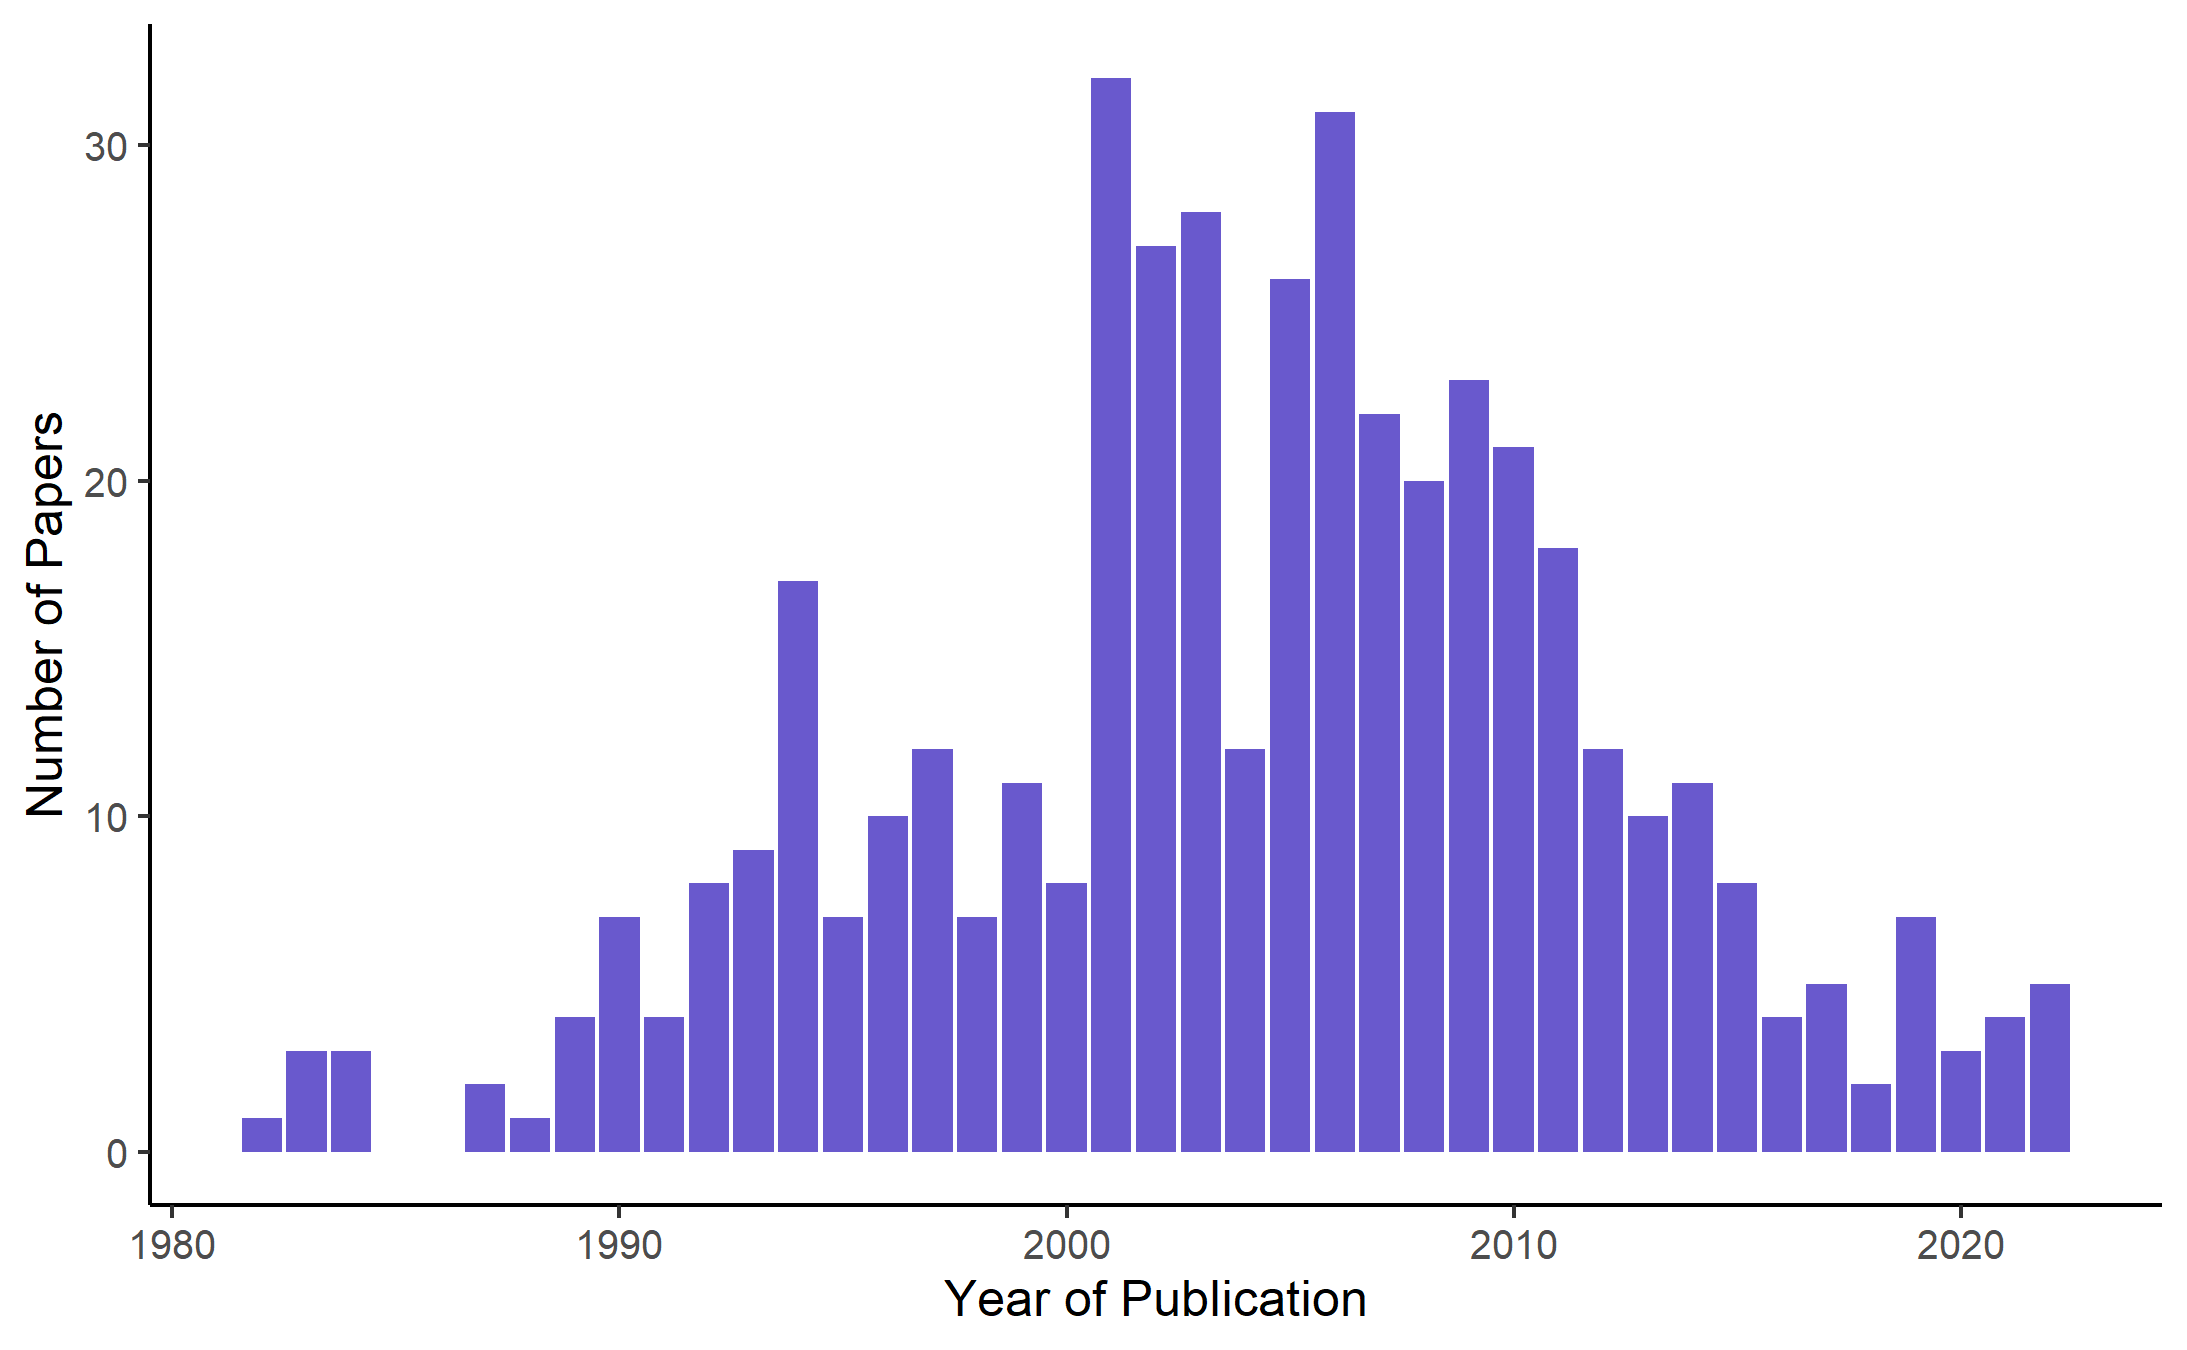
\includegraphics[width=0.8\linewidth]{Figures/Dryland Salinity Papers} \caption{Number of papers on the Web of Science related to the search terms (Dryland Salinity) AND Australia, 1980 - 2022}\label{fig:SalinityPapers}
\end{figure}

The poor spatial and timescale distribution of water quality datasets
has long been an obstacle to measuring trends in salinity. Studies such
as Jolly et. al. \citeyearpar{Jolly2001} and White et. al
\citeyearpar{White2009} used large historical datasets to detect
broadscale trends over large periods throughout the Murray Darling Basin
(MDB). This work identified that southern and eastern dryland regions in
the Murray Darling Basin have rising salinity trends that were worse in
areas of low rainfall \citep{White2009, Jolly2001}. However, the ion
composition varied greatly throughout the Murray Darling Basin (MDB)
\citep{White2009}. More specifically, Conyers et al.
\citeyearpar{Conyers2008} tried to isolate which areas in the middle
portion of the Murrumbidgee catchment acted as sources of salinity, as
well as whether this was predominantly marine cyclic salts (NaCl) as
previously assumed, or whether salts from mineral weathering were also
involved (e.g.~Ca, Mg, HCO\textsubscript{3}). While both are captured in
the bulk measurement of electrical conductivity (EC), a rise in marine
cyclic salts can be a major source of osmotic stress, whereas mineral
weathering salts are far less harmful and are more likely to precipitate
at reasonably low concentrations \citep{Conyers2008}. The ratio of
Cl:HCO\textsubscript{3} ions was identified as the best indicator of the
source of salinity, with Cl\textsuperscript{-} acting as a measure of
marine cyclic salts and HCO\textsubscript{3}\textsuperscript{-} acting
as a measure of mineral weathering salts. The Muttama catchment was
specifically identified as a candidate for future research as ion
concentrations appeared to result in a change from east to west,
correlating with the underlying geology and their mineral composition.

It is clear from these examples that detailed spatial and temporal
datasets are key to understanding different hydrogeochemical processes
in the landscape \citep[e.g.][]{Cartwright2010, Dalhaus2010}, but
overall publicly available datasets on dryland salinity in Australia
remain limited to detailed data from small experimental catchments
(\textless{} 100 ha) \citep{Summerell2006, crosbie2007, Hughes2007} or
sparse government datasets from official monitoring
(i.e.~\href{https://waterinsights.waternsw.com.au/}{WaterNSW
WaterInsights platform}) which tend to be limited in hydrogeochemical
data. Part of this is related to the sensitivity of the data given the
relationship with possible land values. However, as the understanding of
salinity occurrence grows, this argument is less valid. Making data more
widely available would increase the opportunities for research and
increase our understanding of dryland salinity processes.

Without regular and expensive automated sampling, field campaigns to
collect water quality data tend to be ``snapshot'' activities
\citep{Grayson1997, Breuer2015, Lyon2008, Cartwright2010, Lintern2018}
which can be biased due to the over representation of low flow
conditions \citep{Lessels2020}. Even the analyses of substantial
government databases \citep{Lintern2018} are likely to be biased in this
way. This means that overall there are limited streamflow and
groundwater salinity data sets that combine multiple locations across a
significant time period and that combine a range of flow
characteristics.

The aim of this paper is to present and describe the space time
dimensions and basic relationships of a complex groundwater and surface
water hydrogeochemistry dataset that was collected over a 14 year period
in a 1000 km\textsuperscript{2} agricultural catchment in New South
Wales, Australia. The Muttama catchment, which is the focus of this
paper, provides a microcosm of groundwater and surface water salinity
variability in Australia. Focusing on a medium size catchment in greater
detail creates opportunities to test whether sources of salinity can be
traced back to specific areas of land. The Muttama catchment is
representative of flat semi-arid catchments globally, but especially of
Australian catchments, where a significant amount of research has taken
place at the catchment scale
\citep[e.g.][]{crosbie2007, Hughes2007, hughes2008, Summerell2006}.
Unfortunately, a lot of the older data is not easily accessible and
extractable. This paper attempts to correct this by providing an open
dataset, which hopefully will also encourage other research teams to
summarise and report open data. We believe that the data would be
relevant for semi-arid areas in the US, Canada, Asia and South America
\citep{thorslund_vanvliet2020, stavi2021}.

This paper gives a description of the dataset to facilitate open access
of the dataset, but does not analyse the physiochemical relationships in
the data in detail. This will be analysed in follow-up papers and was
partly analysed in an earlier thesis \citep{Akter2018}. The main aim of
this paper is to make the data set accessible to other researchers to
encourage further research in this catchment and in salinity in general.

\section{Methods}

\subsection{Muttama catchment}

The 1000 km\textsuperscript{2} Muttama creek catchment (Figure
\ref{fig:samplemap}) is located in the Mid-Murrumbidgee catchment area
of NSW in south eastern Australia. The landscape is undulating with
elevation variations ranging from 227 - 719 m. Muttama creek flows
north-south through the length of the catchment towards the Murrumbidgee
River near Gundagai. The main township, Cootamundra is located in the
upper half of the catchment. The dominant land use type of this
catchment is about 93\% agriculture, dominated by winter-spring cropping
and pasture. Mean annual rainfall (1891-2024) in the catchment is 654 mm
for the longest running Bureau of Meteorology Landgrove station (station
073022), while potential evapotranspiration far exceeds this total.

Streamflow is measured continuously by WaterNSW, the state agency
responsible for water data collection, at three locations in the
catchment: Coolac, station no. 410044, the main downstream point, and
Berthong, station no. 41000207 and Jindalee, station no. 410112 on two
branches above the Cootamundra township. These data are available as
open access via the
\href{https://waterinsights.waternsw.com.au/}{WaterNSW WaterInsights
platform} or through the \href{http://bom.gov.au/waterdata/}{Bureau of
Meteorology}. Here, we only use the data from the Coolac station as a
comparison.

\begin{figure}
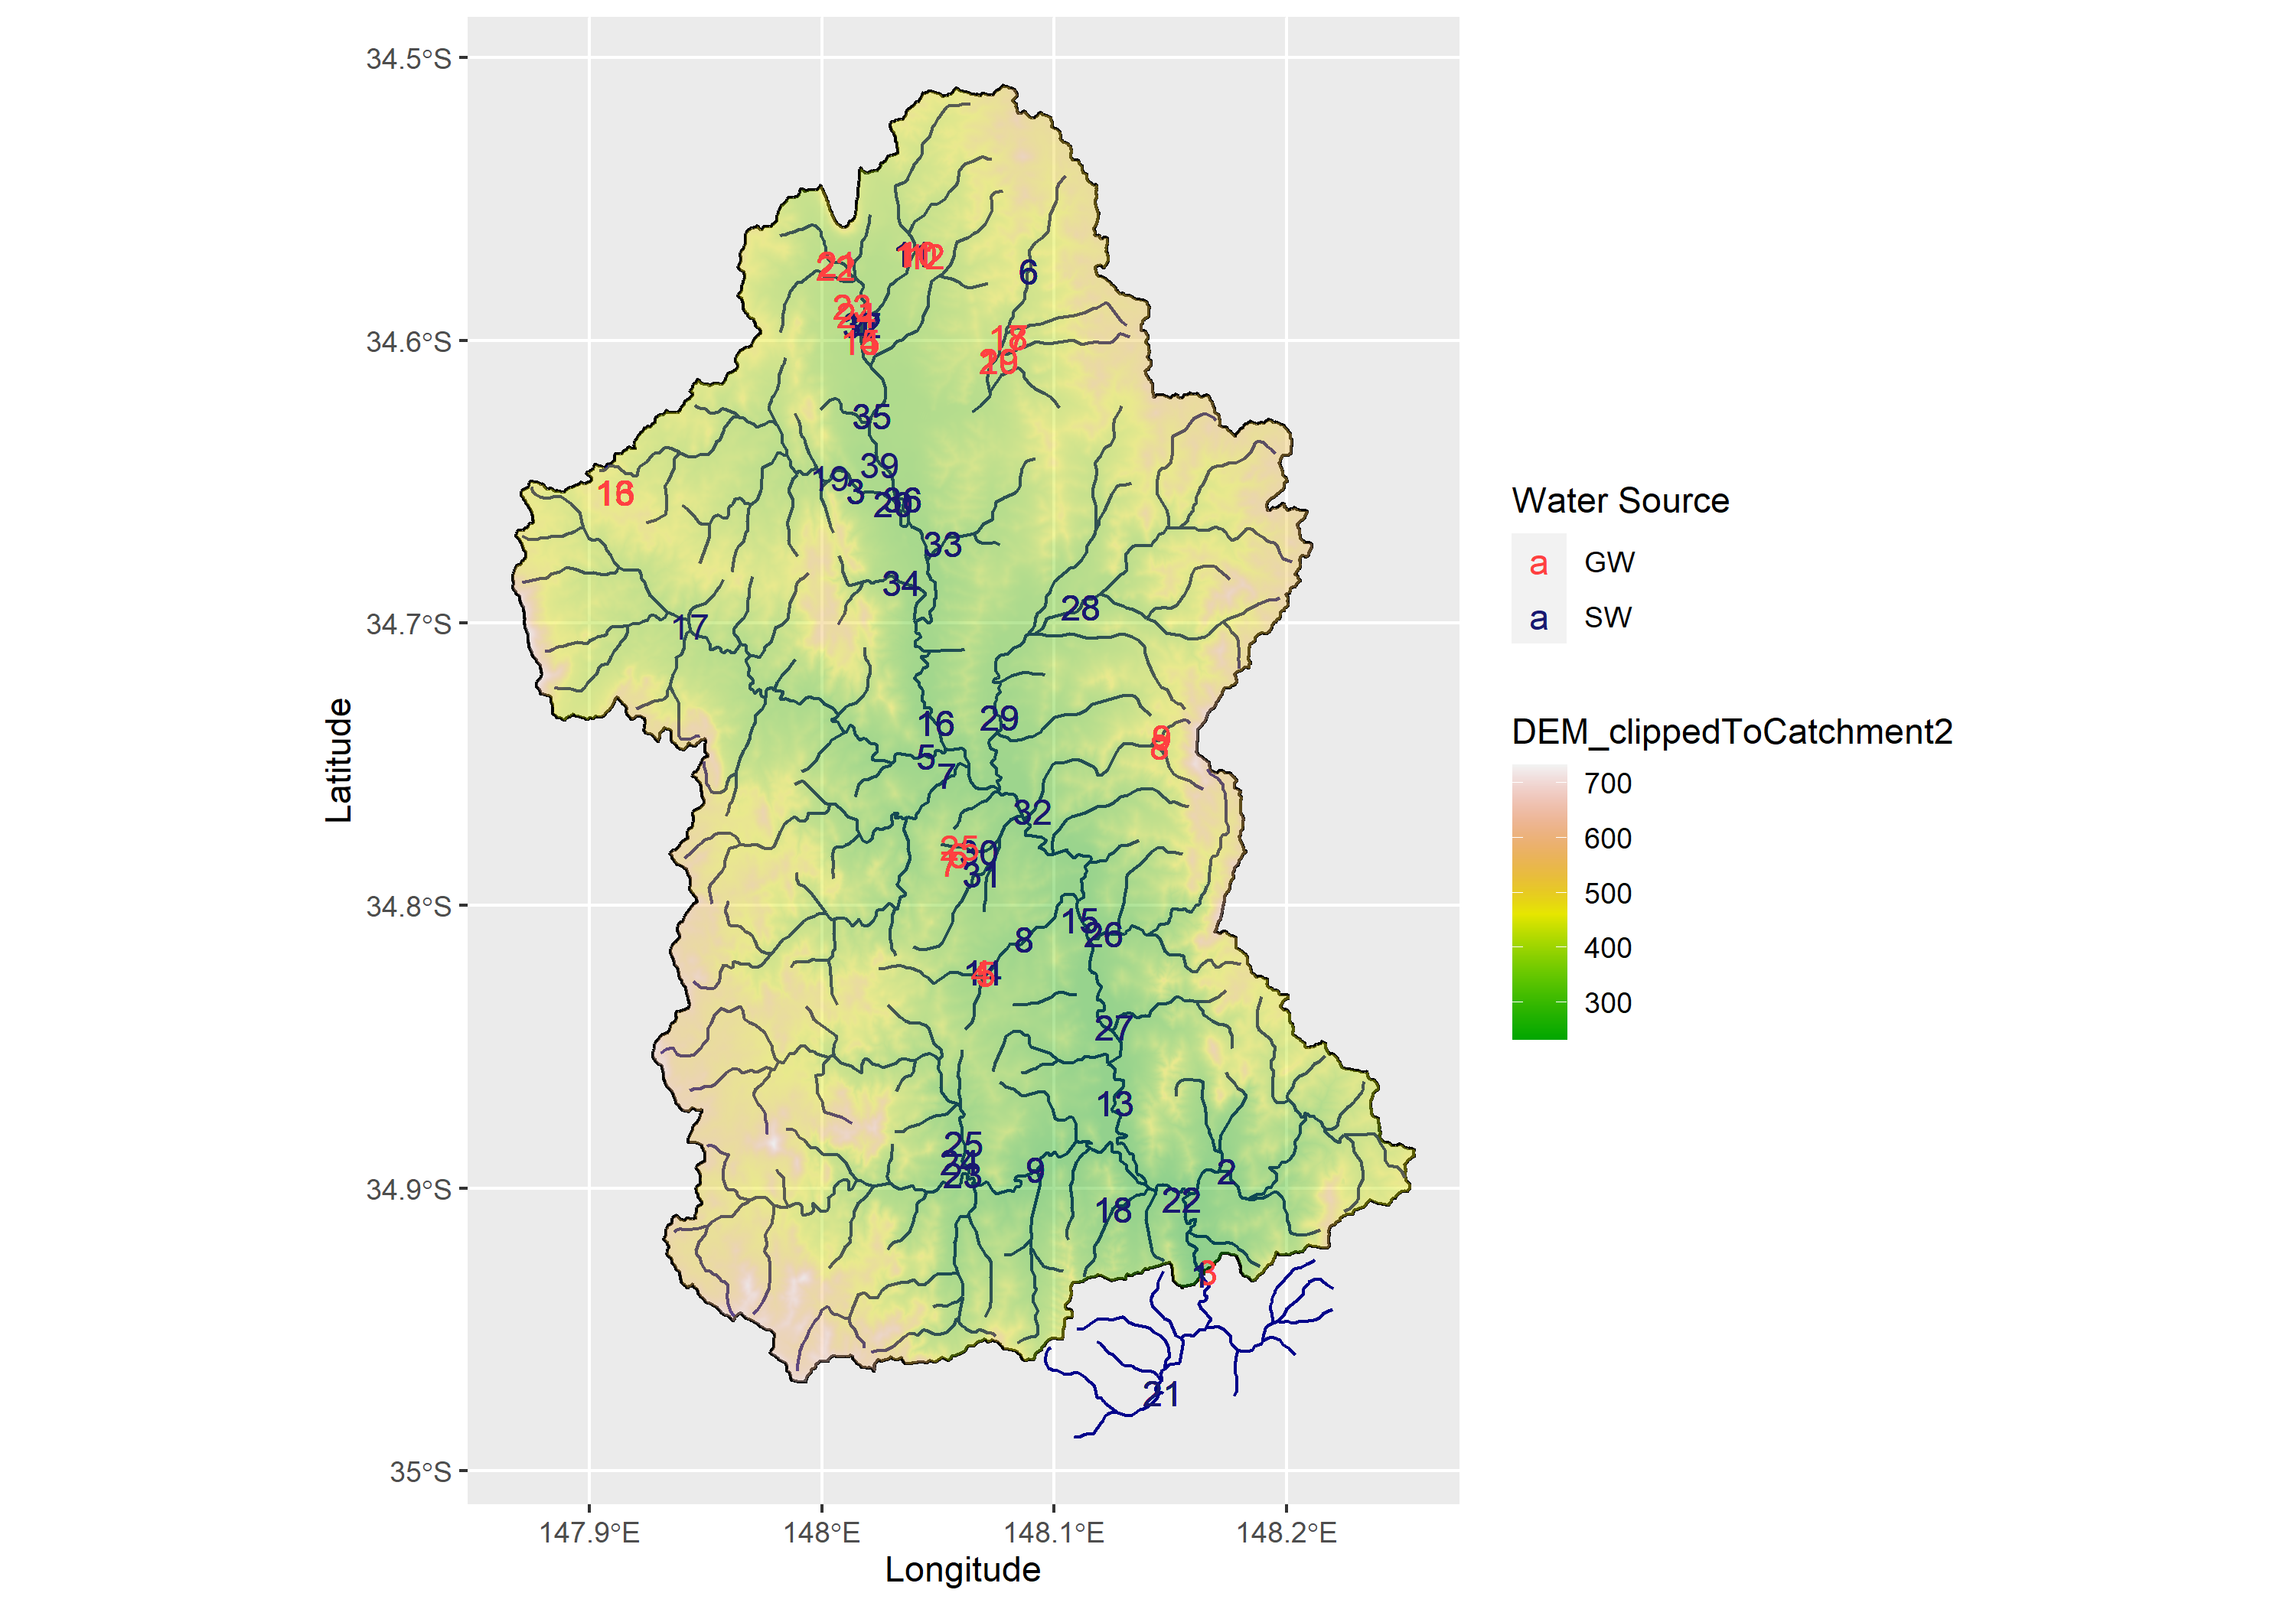
\includegraphics[width=0.8\linewidth]{Figures/gw_or_sw_map} \caption{Muttama Catchment Sampling Locations with Elevation. Symbol colour indicates whether location was a groundwater or surface water source, with blue being surface water and coral red being groundwater. The numbers on the map represent the sample location number.}\label{fig:samplemap}
\end{figure}

The depth to the nearest groundwater table varies across the Muttama
catchment and it ranges from \textless{} 2 m to 20 m below ground level
\citep{DECC2009}. Deep groundwater in the catchment occurs mostly in
fractured rock aquifers common on the eastern, and western fringes of
the catchment. In contrast, shallow groundwater is associated with
unconfined alluvial, colluvial, and eluvial aquifers. Some aquifers in
the northern part of this catchment show artesian behavior
\citep{Webb1999, Akter2018}.

Saline areas of the catchment tend to be associated with geological
heterogeneity, primarily the sedimentary materials in the west and
rhyolite on the northwest side \citep{Conyers2008}. Overall, Muttama
creek is a significant salt contributor to the downstream Murrumbidgee
river with suggested contributions of around 58\% from cyclic sources
and 42\% salts originating from mineral weathering \citep{Conyers2008}.

\subsection{Data Collection}

\subsubsection{Data Sources}

The water quality dataset contains data from 4 main sampling sources
related to four distinct groups of ``people'' doing the sample
collection. The term ``people'' is used loosely, as it mainly related to
four different types of sampling campaigns, which potentially had
differences in the rigour of the sampling campaign (quality control,
types of samples taken, training of the people taking the samples).
These groups are designated as:

\begin{itemize}
\item
  Source 1: Data from the PhD study by Akter \citeyearpar{Akter2018}.
\item
  Source 2: Data from the sampling campaign of two former students, the
  PhD from Lessels \citeyearpar{Lessels2014} and unpublished data from
  another student, E. Milne.
\item
  Source 3: A dataset collected by undergraduate and postgraduate
  students as part of field trips in different units of study at the
  University of Sydney is identified as ``Student data''. This data was
  sampled ``ad-hoc'' during the field trip period using standard
  sampling protocols as described for the data from Akter
  \citeyearpar{Akter2018}.
\item
  Source 4: Data from several autosamplers installed in the catchment
  during the PhD from Lessels \citeyearpar{Lessels2014}. Because these
  samples were not taken by a ``person'' and were taken on a flow
  weighted basis, we separated the data from the ``grab'' samples in the
  other methods. These samples are also missing field measurements, as
  these were only analysed in the laboratory.
\end{itemize}

Overall, 1160 water samples were collected from 62 sample locations over
the 2010 - 2024 period. However, not all sites were sampled at all times
and not all samples were fully analysed for all hydrogeochemical
variables. Both surface water and groundwater samples were collected at
23 groundwater sample sites and 39 surface water sites. These are
distributed across the catchment, depending on standing water
availability and access.

In addition to the water quality dataset, data from 23 groundwater data
loggers is provided from the same groundwater sample sites as in the
hydrogeochemical dataset.

\subsubsection{Hydrogeochemical Variables}

The overall structure of the hydrogeochemical dataset consists of
repeated measurements over time at multiple locations in Muttama
catchment. For each location the name of the location and the spatial
coordinates were recorded in decimal degrees (Longitude = x and Latitude
= y) as well as whether the location was a groundwater or a surface
water location. The names of the locations are fairly random and basic
locality indicators, which cannot be interpreted exactly.

The data for each location consist of up to six variables which were
measured in the field (Table \ref{tab:TableMeasurements}). These were
complemented by laboratory analysis, which repeated some of the field
measurements, and for additional major anion and cation variables (Ca,
Mg, Na, K, Cl, SO\textsubscript{4}, HCO\textsubscript{3}), and total
Nitrogen (N) and total Phosphorus (P) for part of the sample set. Some
other variables were infrequently measured and are not included in the
data set.

\begin{table}
\centering
\caption{\label{tab:TableMeasurements}Variables measured in the field and laboratory.}
\centering
\resizebox{\ifdim\width>\linewidth\linewidth\else\width\fi}{!}{
\begin{tabular}[t]{l|r|l|l|l|l|l|l|l|l}
\hline
Field measurements & Records Field & Lab repeat & Records Lab & Anions & Records Anions & Cations & Records Cations & Other & Records other\\
\hline
pH & 742 & pH & 182 & Cl$^-$ & 1010 & Na$^+$ & 1035 & Total Nitrogen & 96\\
\hline
EC (Electrical conductivity) & 274 & EC & 332 & HCO$_3^-$ & 583 & Mg$^{2+}$ & 1035 & Total Phosphorus & 96\\
\hline
SPC (temperature corrected EC) & 653 &  &  & SO$_4^{2-}$ & 961 & K$^+$ & 1035 &  & \\
\hline
Temperature & 684 &  &  &  &  & Ca$^{2+}$ & 1035 &  & \\
\hline
Dissolved Oxygen (DO) & 174 &  &  &  &  &  &  &  & \\
\hline
Turbidity & 90 &  &  &  &  &  &  &  & \\
\hline
\end{tabular}}
\end{table}

The variables pH, EC, SPC (specific conductance: field temperature
corrected EC), Temperature, and in some cases dissolved oxygen (DO) and
Turbidity were measured using a range of field probes (Table
\ref{tab:TableInstruments}). All field probes measured pH, EC,
Temperature and calculated SPC. Early measurements (samples up to
November 2014) used a YSI probe that included a turbidity and DO probe
(YSI 6600 and YSI 600 for surface and groundwater, respectively). Later
groundwater samples (After November 2014) used a different YSI probe
(YSI ProDSS multi-parameter) that only included a DO probe, while the
suface water sampling used a YSI EXO2 multiparameter sonde that included
pH, EC, DO and Turbidity. Finally, (after mid 2019) surface water and
groundwater sampling used a Xylem Exo probe with DO, pH, EC, Temperature
and SPC. Some of the variability in the field measurements might be due
to this variation in the field instrumentation.

\begin{table}
\centering
\caption{\label{tab:TableInstruments}Different instruments used in the sampling.}
\centering
\resizebox{\ifdim\width>\linewidth\linewidth\else\width\fi}{!}{
\begin{tabular}[t]{>{}l|l|l|l}
\hline
Instrument & Purpose & Date & Sensors\\
\hline
\textbf{YSI6600} & Surface water & up to November 2014 & pH: 6561 pH probe\\
\cline{4-4}
 &  &  & Temperature/EC: 6560 Conductivity/Temperature\\
\cline{4-4}
 &  &  & Turbidity: 6136 Turbidity Probe, Wiping\\
\cline{4-4}
 &  &  & DO: 6562 Dissolved oxygen probe\\
\cline{1-2}
\cline{4-4}
\textbf{YSI600} & Ground water &  & pH: 6561 pH probe\\
\cline{4-4}
 &  &  & Temperature/EC: 6560 Conductivity/Temperature probe\\
\cline{1-1}
\cline{3-4}
\textbf{YSI ProDSS multiparameter sampling} &  & November 2014 - mid 2019 & pH: ProDSS pH Sensor with Module\\
\cline{4-4}
 &  &  & Temperature/EC: ProDSS Conductivity and Temperature Sensor\\
\cline{4-4}
 &  &  & DO: ProDSS ODO Optical Dissolved Oxygen Sensor\\
\cline{1-4}
\textbf{YSI EXO2 multiparameter sonde} & Surface water & After November 2014 - end 2023 & pH:EXO pH Smart Sensor\\
\cline{4-4}
 &  &  & Temperature/EC: EXO Conductivity and Temperature Smart Sensor\\
\cline{4-4}
 &  &  & Turbidity: EXO Turbidity Smart Sensor\\
\cline{4-4}
 &  &  & DO: EXO Optical Dissolved Oxygen Smart Sensor\\
\cline{1-4}
\textbf{YSI EXO1 multiparameter sonde} & Ground water & After Mid 2019 to current & pH: EXO pH Smart Sensor\\
\cline{4-4}
 &  &  & Temperature/EC: EXO Conductivity and Temperature Smart Sensor\\
\cline{1-4}
\textbf{YSI ProDSS multiparameter sampling} & Surface water & Start 2024 to current & pH: ProDSS pH Sensor with Module\\
\cline{4-4}
 &  &  & Temperature/EC: ProDSS Conductivity and Temperature Sensor\\
\cline{4-4}
 &  &  & Turbidity: ProDSS Turbidity Sensor\\
\cline{4-4}
 &  &  & DO: ProDSS ODO Optical Dissolved Oxygen Sensor\\
\hline
\end{tabular}}
\end{table}

Anions in most of the samples were analysed using the high-performance
liquid chromatography method (Dionex P680 HPLC) and cations were
measured on acidified samples using an Inductively Coupled Plasma
Optical Emission Spectrometer (ICP-OES, Varian 720-ES) at the University
of Sydney \citep{Akter2018}. Duplicate samples in the analysis had a
reported relative percentage difference (RPD) lower than 5\% in part of
the sample dataset \citep{Akter2018}. Some of the later samples and the
student sample set (Source 3) were analysed by a commercial laboratory
(\href{https://www.alsglobal.com/en/locations/asia-pacific/pacific/australia/nsw/sydney-woodpark-environmental}{ALS
Environmental, Smithfield, NSW}). Alkalinity concentrations were
generally measured in the field within 24h of collection using a HACH
digital titrator (model 16900) \citep{Akter2018} up to 2017 and by the
commercial laboratory after this.

The hydrogeochemical data is stored on the University of Sydney
escholarship repository: \url{doi.org/10.25910/m0wp-8890}

\subsection{Continuous variables}

The logger data, which early on collected groundwater pressure levels at
15 min and from mid-2016 at 2 hour intervals, were adjusted for the
length of the cable and the height of the standpipe above the ground
level. They were subsequently summarised to raw daily values using an R
script (\texttt{SummariseDailyData.R}), which is stored with the raw
data in the Open Science Foundation (OSF) repository associated with
this paper \url{https://doi.org/10.17605/OSF.IO/BEUWK}.

The loggers in the field were uncalibrated. Due to logger failures, gaps
occur in the daily data, followed by replacement of the faulty loggers.
In some cases the cable length was adjusted and this was recorded in the
field notes. Overall, this resulted in data with gaps and sometimes
shifts in the recorded logger data.

Manual water level measurements were taken at each manual sampling date
to allow calibration of the logger data. To correct the groundwater
logger data, the daily data was matched to the observed data using
linear regression, if more than 3 manual observed data were available
and slope and intercept of the regression had a p-value \textless{} 0.1.
If there were less than 3 manual observed data points for the specific
logger an adjustment to the data was based on the difference between the
average observed data and the average recorded water levels. Otherwise
no adjustment was made. After the manual observations are made, the well
is purged and the logger is temporarily removed from the well. This data
(during the temporarily removal of the logger during the purging and
subsequent recovery of the groundwater level) is removed from the logger
data series. As a result, there is no direct time match between the
logger data series and the manual observations. However, the data showed
that, in most cases, the groundwater level recovered within 24 hrs. The
pseudo code in the supplementary material describes the process in more
detail.

The code used to match the manually observed data with the logger data
is in the script \texttt{Match\_obs\_logger\_data.R}, which is stored
with the raw data in the Open Science Foundation (OSF) repository
associated with this paper \url{https://doi.org/10.17605/OSF.IO/BEUWK}.

After the automated process, two of the groundwater level data series
still had substantial discrepancies in some sections of the data. This
was most likely due to a lack of observed data for the specific logger.
A final manual correction was applied. As this process is based on
judgement of the data by the authors of this paper, we documented this
in detail in the supplementary material.

The final corrected data that is published with this paper on
\url{https://doi.org/10.17605/OSF.IO/BEUWK} includes a column which
describes whether the data is based on the automatic correction or a
further manual correction.

\clearpage

\subsection{Boxplots and maps}

Using the most complete data, boxplots and spatial maps were generated
to highlight the spatial and temporal variation in the data set. The
boxplots visually highlight empirical differences in the data.

The mean concentration and interquartile range (25\textsuperscript{th} -
75\textsuperscript{th} percentile) of the concentration data
distributions were calculated to give an indication of variation of the
data in the spatial maps.

All graphs and maps were produced using R version 4.3.1 \citep{R2023}.
All code can be found in the associated
\href{https://github.com/WillemVervoort/MuttamaDataPaper}{github
repository}, as part of the markdown document for this paper.

\section{Results}

\subsection{Distribution of missing Values}

\begin{figure}
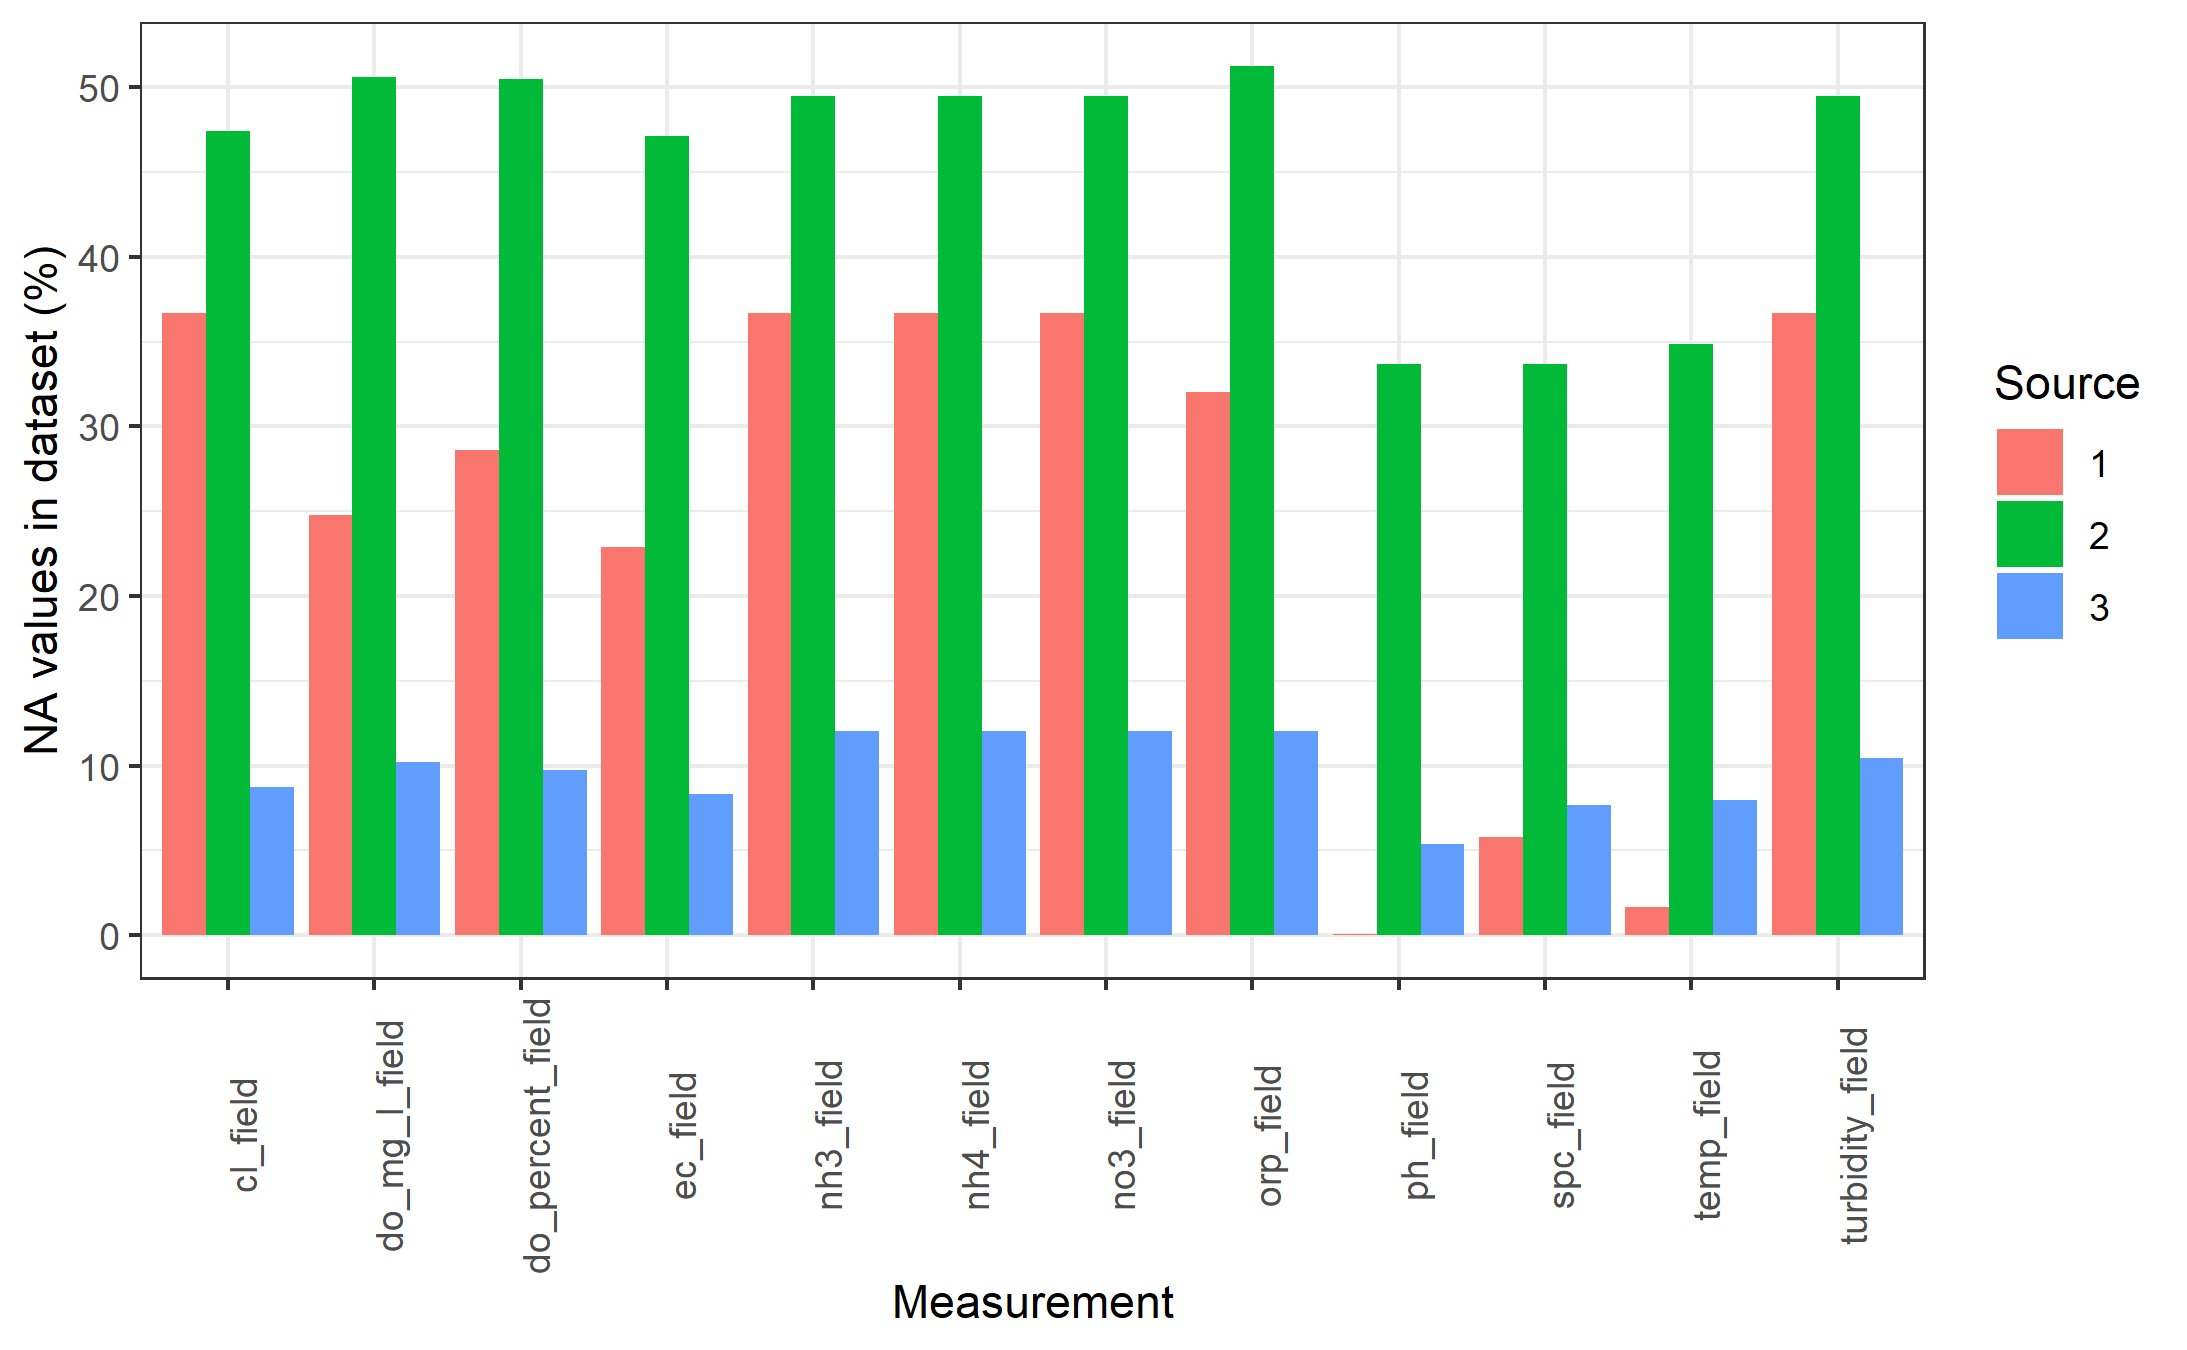
\includegraphics[width=0.9\linewidth]{Figures/na_count} \caption{Top: Distribution of missing values for the different data sources and measurement types. Most of these missing values were because not all the variables were analysed for all the samples, see the explanation in the article text. Bottom: Percent missing values for the groundwater data across all piezometers, summarised by month.}\label{fig:na-plot}
\end{figure}

In the hydrogeochemistry data, data source 3 was the most complete in
terms of variables analysed, because in this set more variables were
analysed in the commercial lab (Figure \ref{fig:na-plot} top). Some of
the variables analysed in the commercial lab were not analysed with the
equipment at the University of Sydney. However, source 3 had the
smallest number of overall samples. Source 2 has the most incomplete
data points. Source 4 has a very consistent number of missing values,
possibly because not all samples were analysed in the set. For source 2,
the missing data suggests that for many of the samples only a few of the
variables were measured and analysed as highlighted above. In the data
from source 2, almost 50\% of samples are incomplete in terms of the
measurement of all the variables in Table 2. Similarly, source 1 had
more incomplete data, because some of the minor elements were not
analysed. The field recorded variables pH, EC, SPC and Temperature were
the most complete as they were generally measured directly in the field.
Thus the distribution of the NA values in the overall data set is mostly
a reflection of the time period of sampling and the change in
methodology over the 14 years of sampling.

In the groundwater level time series, the missing data relate mostly to
logger failures and the different times that wells were instrumented.
Rather than giving a full breakdown by well location, the overall level
of completeness of the series is displayed (Figure \ref{fig:na-plot}
bottom).

\subsection{Temporal Distribution of Data}

Overall the water quality sampling appears to have a reasonable
distribution across all months (Figure \ref{fig:timedist-plot}),
therefore seasonal trends should be identifiable in the data. Average
rainfall data (1995 - 2022) does not indicate any major seasonal trends,
although there is a slight dominance of rainfall in the early Austral
Spring (months 9 and 10, September and October). This also explains the
higher number of samples because, more sampling trips were organised in
this period, and spatially more channels could be sampled for surface
water. The timing of source 3 (the student data) is the result of the
yearly field trips, which tended to occur at approximately the same time
of the year in early March and late September or early October,
coinciding with the University semester breaks.

\begin{figure}
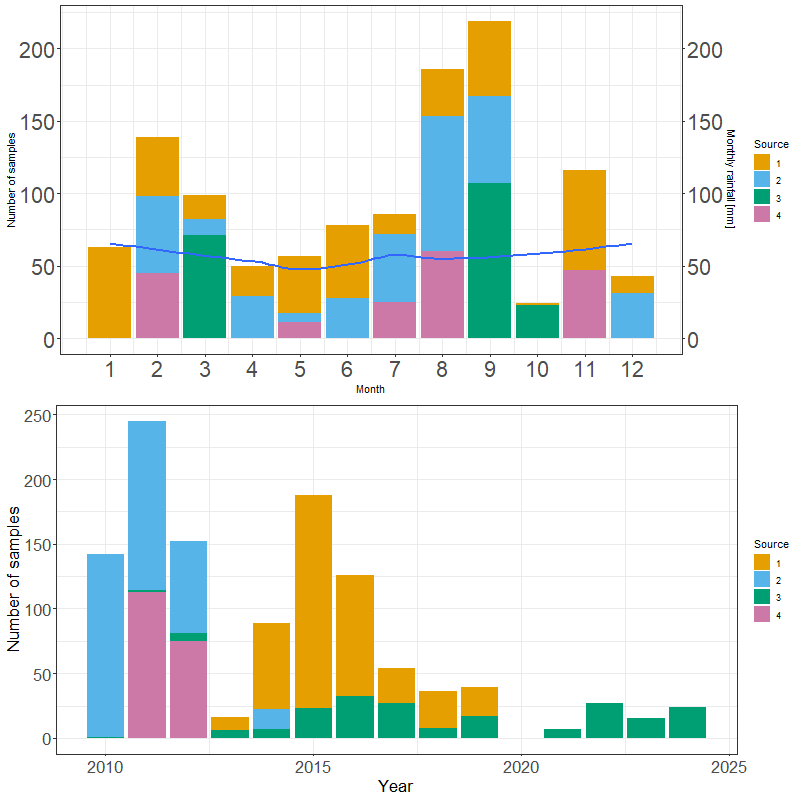
\includegraphics[width=0.7\linewidth]{Figures/timeDist} \caption{Top:Distribution of samples throughout the year (total number of samples collected during each month) with the blue line representing the average monthly rainfall during the study period. Bottom: Distribution of samples over the study period (total number of samples collected during each year).}\label{fig:timedist-plot}
\end{figure}

The number of samples collected in each year relative to the different
sources changes throughout the years reflecting the duration of the
different studies and funding cycles (Figure \ref{fig:timedist-plot});
however the data is still well-distributed enough that overall trends
should be clear. In addition, some of the sample volumes can be related
to the occurrence of rainfall, as in drier years several of the channels
would be dry and no sampling of surface water could occur.

Consistent groundwater sampling commenced later in the project, which
means that there are very few groundwater samples before 2013. In
contrast, the autosamplers were installed early in the project and there
are no samples from this source after 2013.

\begin{figure}
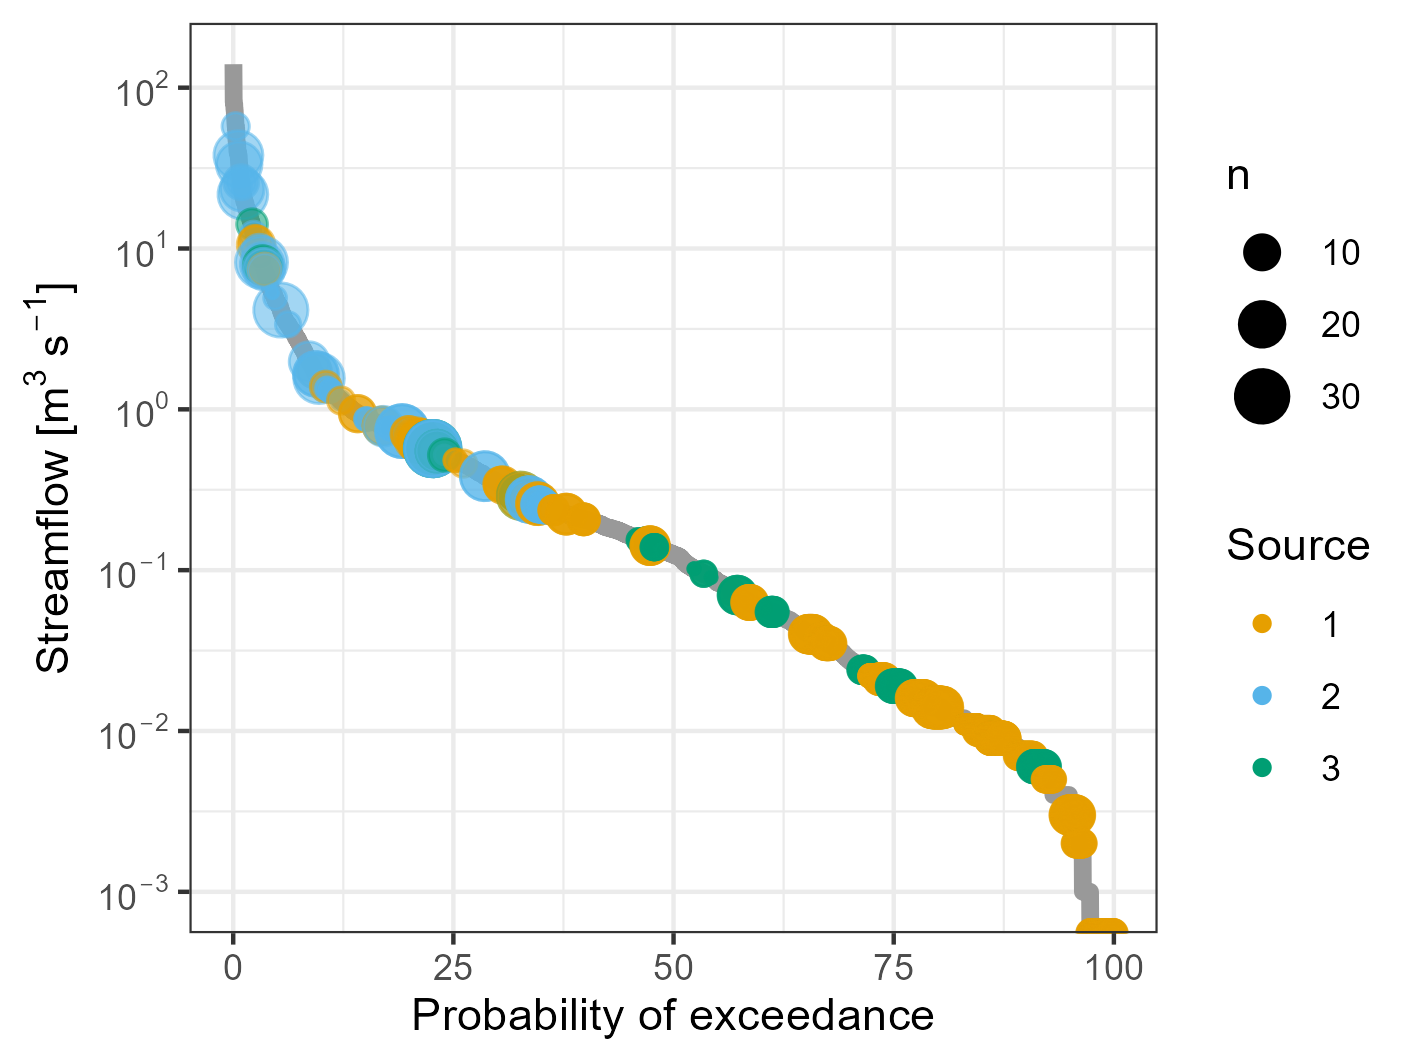
\includegraphics[width=0.8\linewidth]{Figures/FDC} \caption{Sample distribution on flow duration curve derived from flow data at the Coolac NSW government station.}\label{fig:FDC}
\end{figure}

Surface water samples were reasonably well distributed across the flow
distribution, measured at the Coolac station (410044), with only a
possible bias towards periods of medium flow. This is most likely since
many of the upstream surface water sampling points are often completely
dry during periods of low flow at Coolac, and therefore cannot be
sampled. Conversely, there are no manual samples during high or very
high flow as during flood situations sampling was dangerous and
restricted by work health and safety considerations. The samples at high
flow are all from our automated sampling.

\subsubsection{Comparisons of the geochemistry of groundwater samples
with Surface water samples}

\begin{table}
\centering
\caption{\label{tab:TableElementstats}Summary statistics for elements measured in the field.}
\centering
\begin{tabular}[t]{l|l|l|l|l|l|l}
\hline
\multicolumn{1}{c|}{} & \multicolumn{3}{c|}{GW} & \multicolumn{3}{c}{SW} \\
\cline{2-4} \cline{5-7}
Element & Mean & Min & Max & Mean & Min & Max\\
\hline
Temperature field & 17.4 & 11.4 & 30.8 & 15.9 & 4.1 & 32.9\\
\hline
Turbidity field & 30.2 & 0.1 & 90.0 & 13.1 & 0.5 & 51.6\\
\hline
DO field [\%] & 20.1 & -3.2 & 70.7 & 86.8 & 10.4 & 220.2\\
\hline
EC field [µS cm$^{-1}$] & 4006 & 457 & 14385 & 1411 & 117 & 4163\\
\hline
EC lab [µS cm$^{-1}$] & NA & NA & NA & 1292 & 1 & 5230\\
\hline
SPC field & 4667 & 347 & 17799 & 1246 & 61 & 6046\\
\hline
pH field & 7.3 & 6.0 & 8.8 & 8.0 & 6.7 & 10.0\\
\hline
pH lab & NA & NA & NA & 7.6 & 6.8 & 8.5\\
\hline
Cl$^-$ [mg L$^{-1}$] & 1218.3 & 73.0 & 4960.7 & 294.2 & 8.9 & 4577.1\\
\hline
HCO$_3^-$ [mg L$^{-1}$] & 599.5 & 68.0 & 1115.0 & 333.9 & 25.6 & 782.0\\
\hline
SO$_4^{2-}$~[mg L$^{-1}$] & 261.1 & 0.0 & 1319.2 & 48.4 & 0.0 & 987.6\\
\hline
Na$^{+}$ [mg L$^{-1}$] & 492.1 & 17.8 & 2283.7 & 122.1 & 7.1 & 866.2\\
\hline
Mg$^{2+}$ [mg L$^{-1}$] & 167.6 & 6.4 & 654.6 & 66.7 & 1.4 & 276.9\\
\hline
K$^{+}$ [mg L$^{-1}$] & 4.4 & 0.0 & 30.8 & 7.6 & 1.0 & 43.8\\
\hline
Ca$^{2+}$ [mg L$^{-1}$] & 256.4 & 16.3 & 1354.2 & 61.6 & 2.3 & 682.1\\
\hline
TN [mg L$^{-1}$] & 3.7 & 0.6 & 10.3 & 1.2 & 0.0 & 4.9\\
\hline
TP [mg L$^{-1}$] & 0.3 & 0.0 & 1.0 & 0.5 & 0.0 & 5.5\\
\hline
\end{tabular}
\end{table}

The summary of the samples (Table \ref{tab:TableElementstats})
highlights the range of the data for the different variables. Obviously,
surface water will record higher DO values, while groundwater recorded
higher EC and SPC values. The rest of the variables have fairly similar
ranges for both groundwater and surface water. Both total P and total N
are low across the catchment samples, with only a few outliers related
to specific locations and dates.

Groundwater samples have quite a distinctive hydrogeochemical signature
compared to the surface water samples (Figure \ref{fig:gw_sw-plot}).
Since `Source 1' collected most of the groundwater samples, this results
in differences between data collection sources. Field SPC measurements
were used to represent EC since these samples had the fewest missing
data. There also appears to be a slight bias towards lower EC values for
sampling group 2, but this is likely because these samples were
collected during two very wet years in 2010 and 2011 (Figure
\ref{fig:timedist-plot}) and are mostly associated with high flow values
(Figure \ref{fig:FDC}).

\begin{figure}
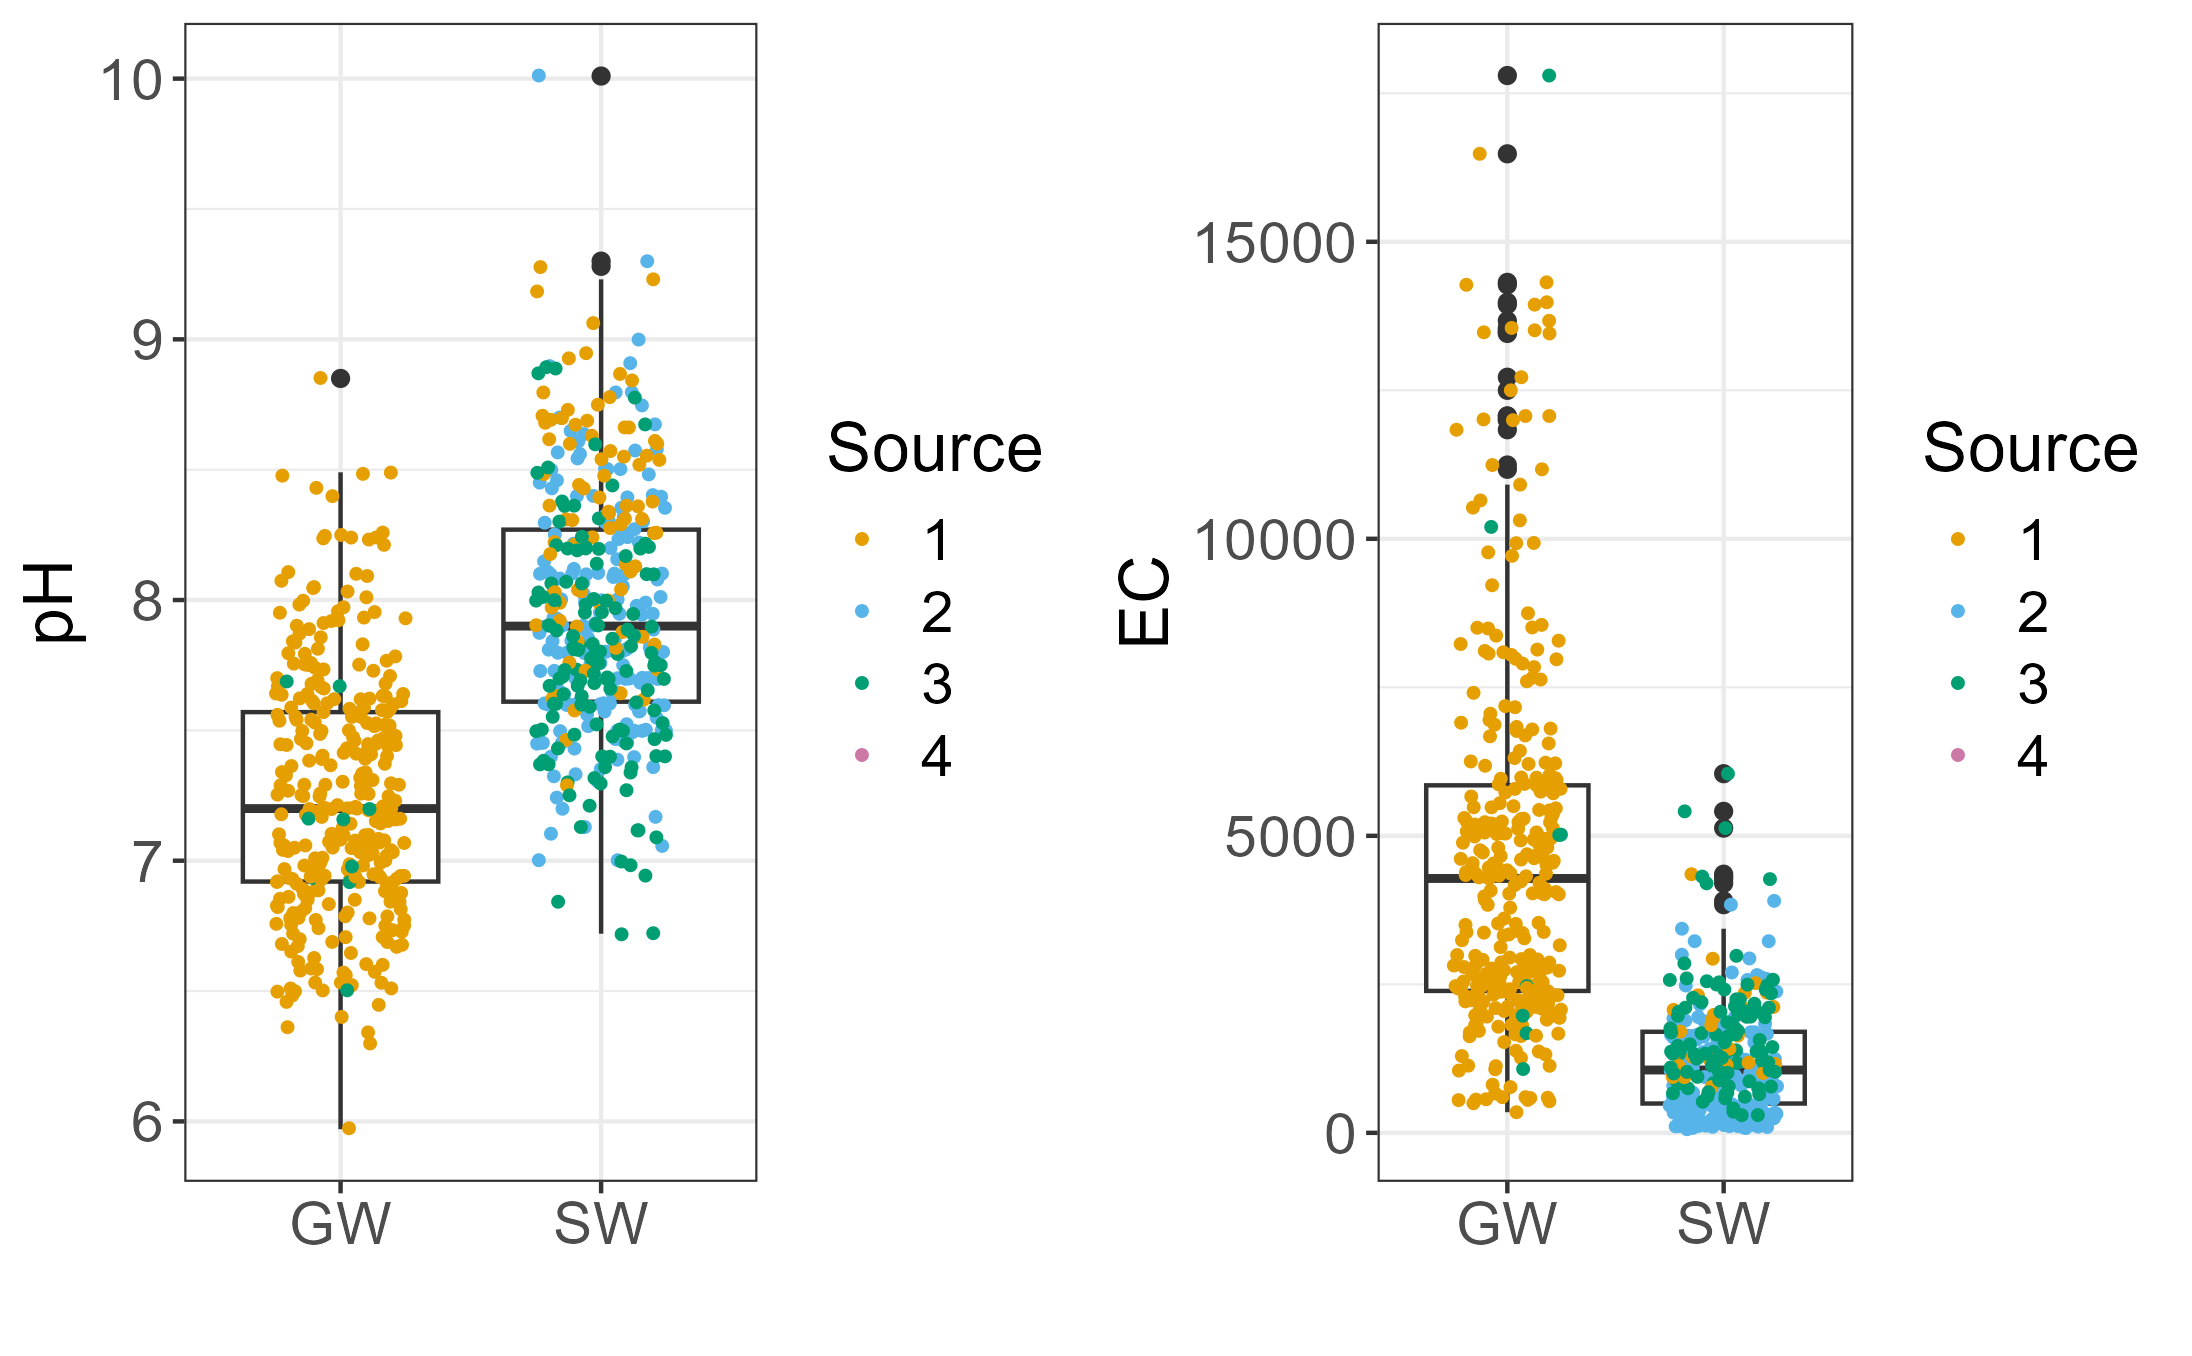
\includegraphics[width=0.8\linewidth]{Figures/gwsw} \caption{Difference in pH and EC for groundwater and surface water samples. The source of the data (the sampling group) is indicated with colour.}\label{fig:gw_sw-plot}
\end{figure}

\subsubsection{Groundwater level data}

\begin{figure}
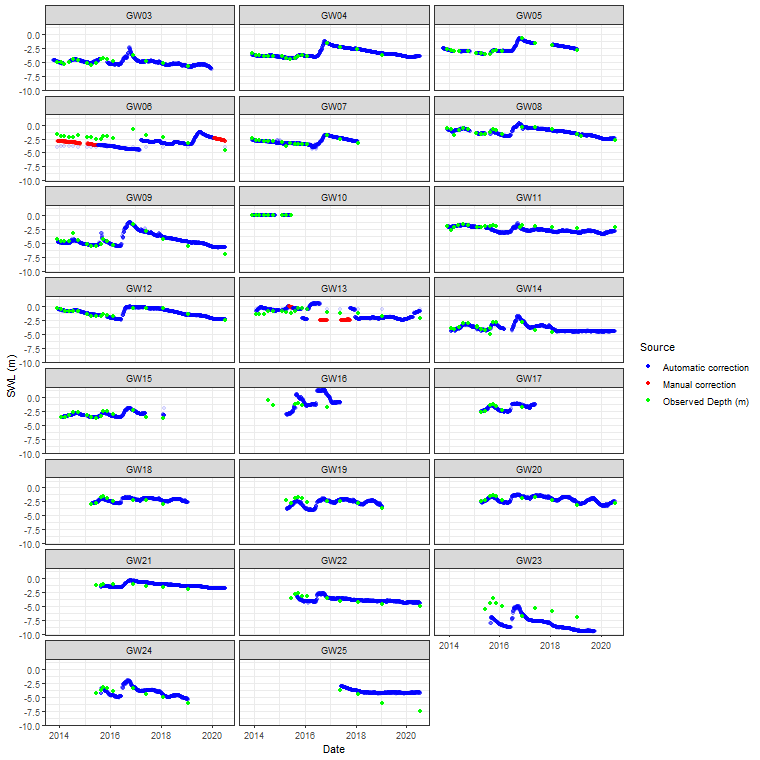
\includegraphics[width=1\linewidth]{Figures/Final_Corrected_piezodepths} \caption{Overview of the corrected groundwater time series for all the wells. Different panels relate to the different locations highlighted in Figure 2.}\label{fig:gw-series}
\end{figure}

The overall corrected groundwater timeseries shows the shorter time that
loggers were installed in the wells (Figure \ref{fig:gw-series}),
associated with the PhD thesis from Akter \citeyearpar{Akter2018}. It
also indicates that the manual data can not always be fully matched with
the logger data, but further corrections are likely to be speculation.

In general, shallow groundwater occurs between 1 and 5 meters below the
surface and is responsive to dry and wet periods. Some of the wells have
positive pressures, resulting in occasional groundwater levels above the
ground surface, such as at GW10, GW12, GW13 and GW21 (Figure
\ref{fig:samplemap} and Figure \ref{fig:gw-series}).

\subsection{Spatial variation}

\clearpage

\begin{figure}
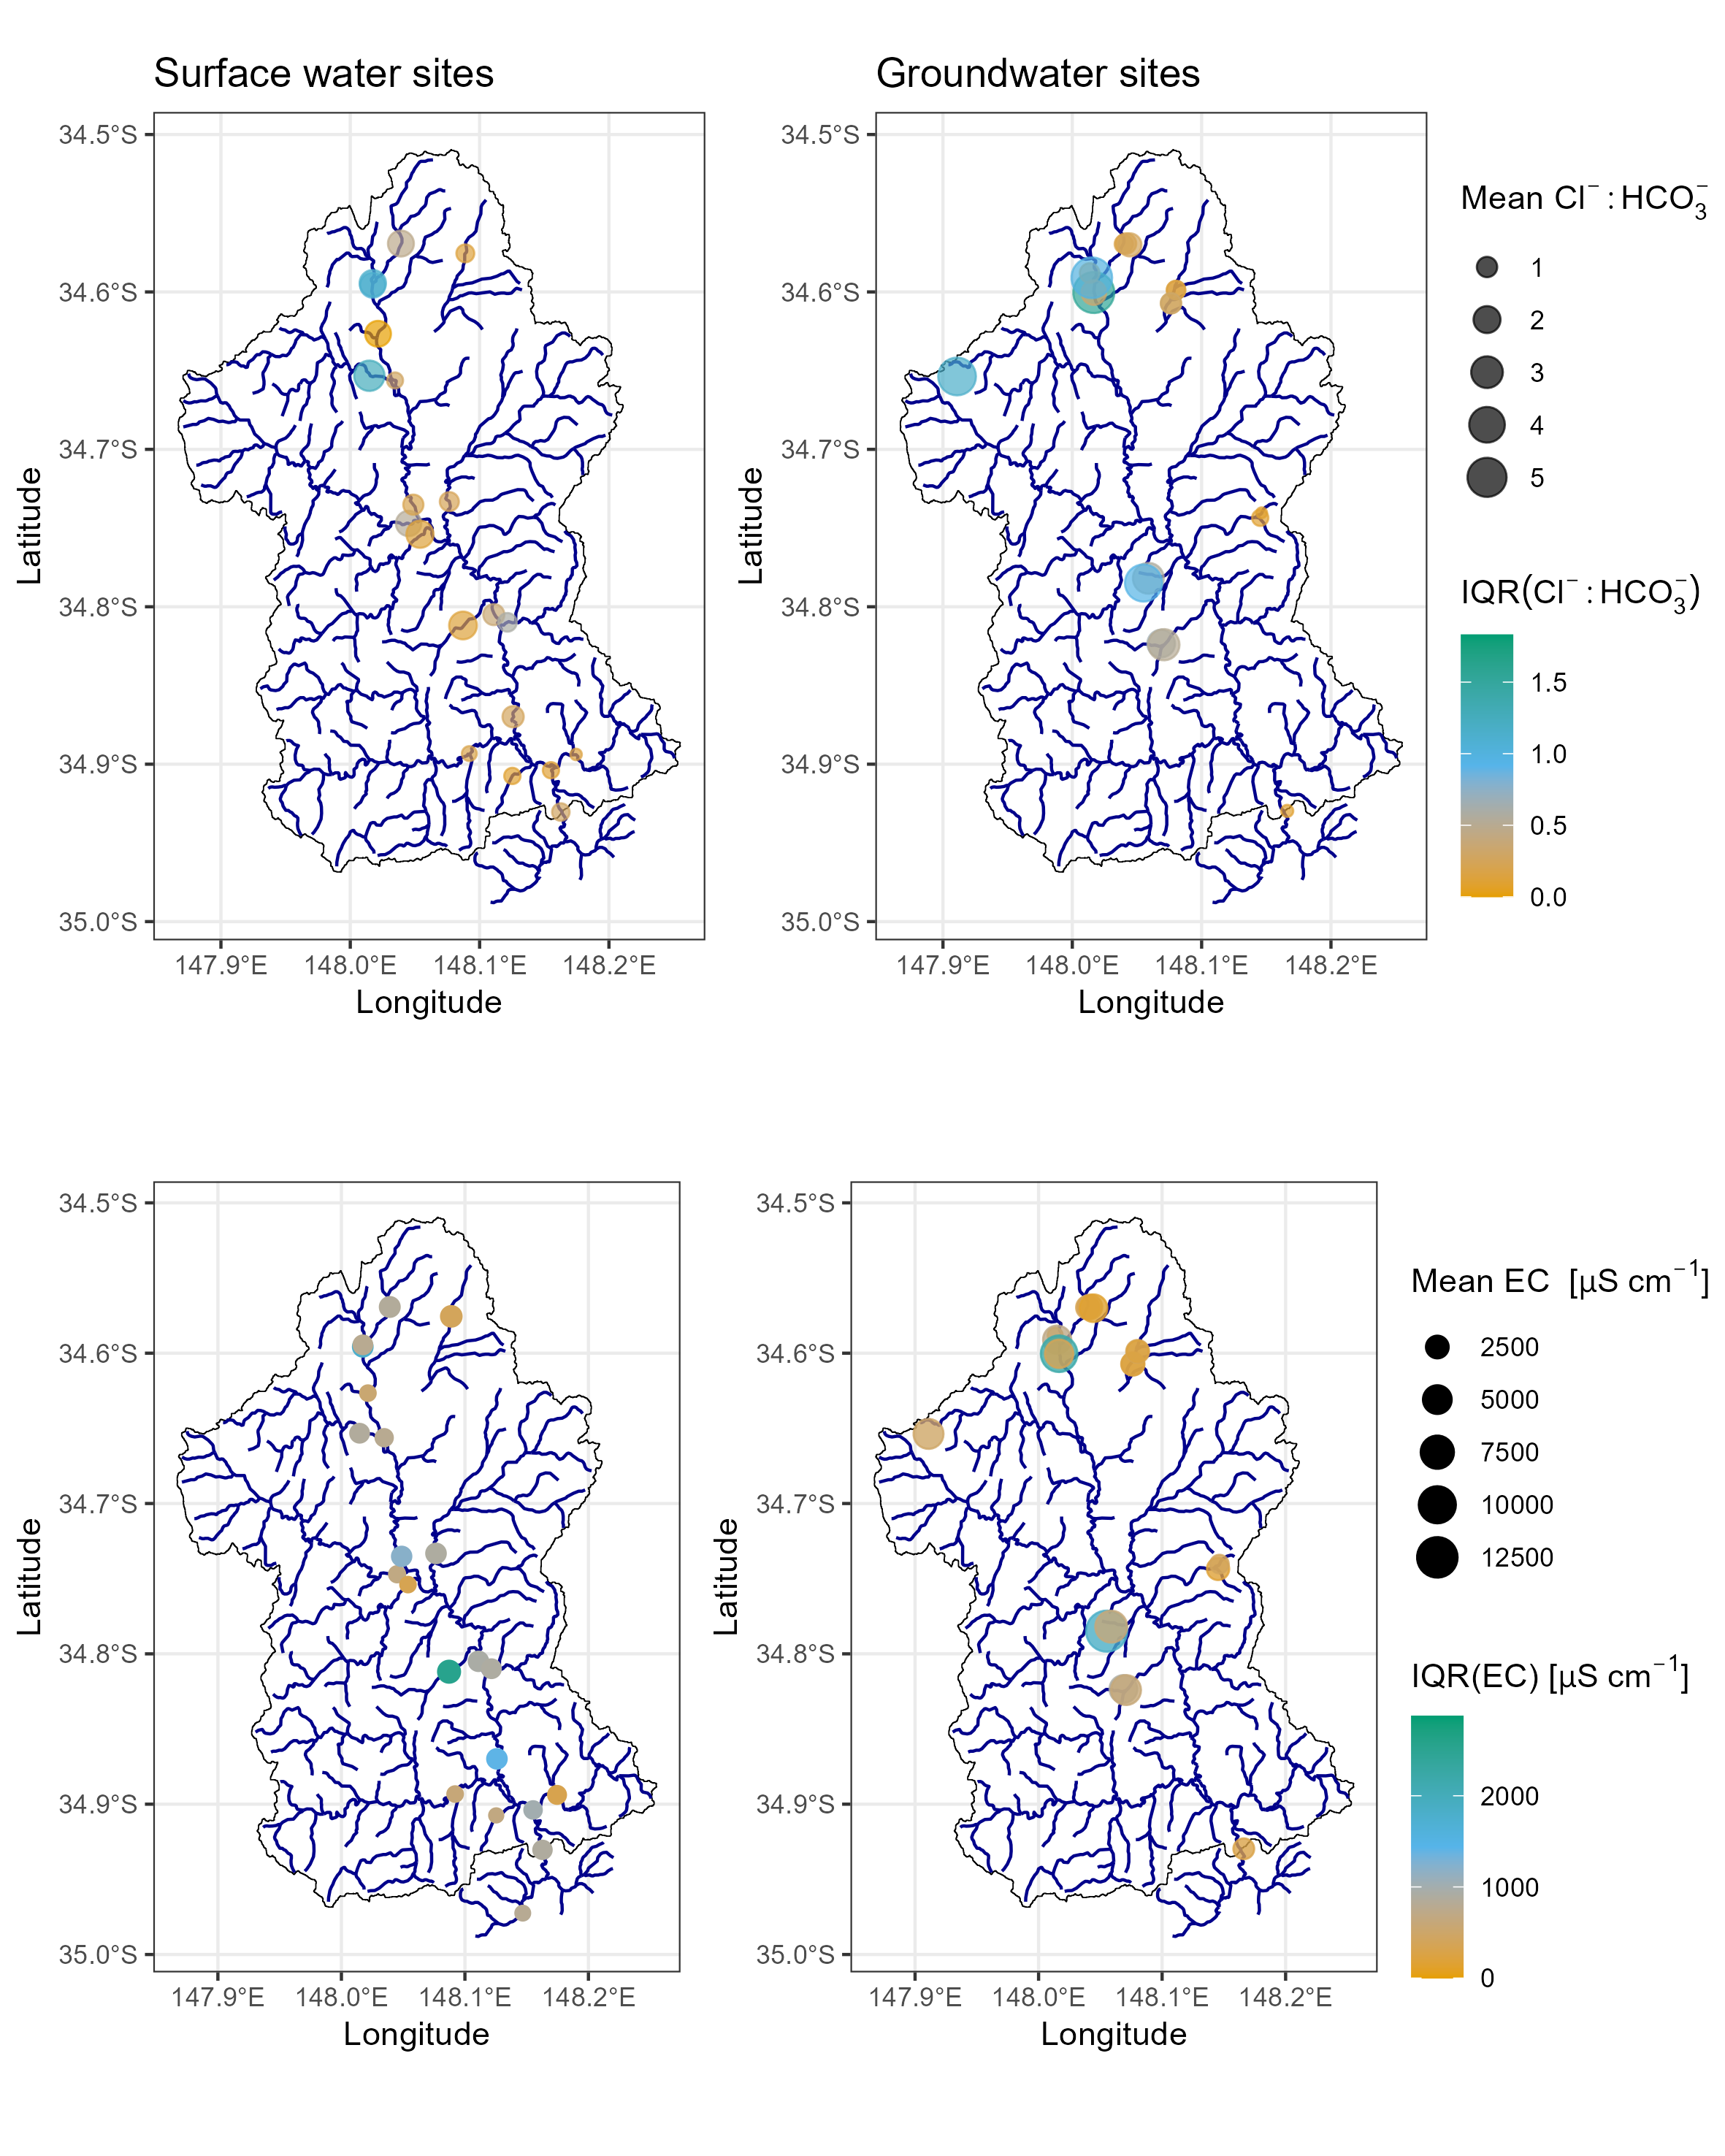
\includegraphics[width=0.8\linewidth]{Figures/spatial_maps} \caption{Top row: Spatial variation of $\mathrm{Cl^-:HCO_3^-}$ ratio throughout the catchment, highlighting mean and interquartile range (IQR) for each sampling location. Bottom row: Spatial Variation of EC throughout the catchment, using Mean EC in $\mathrm{\mu S~cm^{-1}}$ and interquartile range (IQR) for each sampling location. Only locations with more than 10 observations over the 14 years are included. Surface water sample sites are in the left column, while groundwater sample sites are in the right column.}\label{fig:spatial-map}
\end{figure}

\clearpage

\begin{figure}
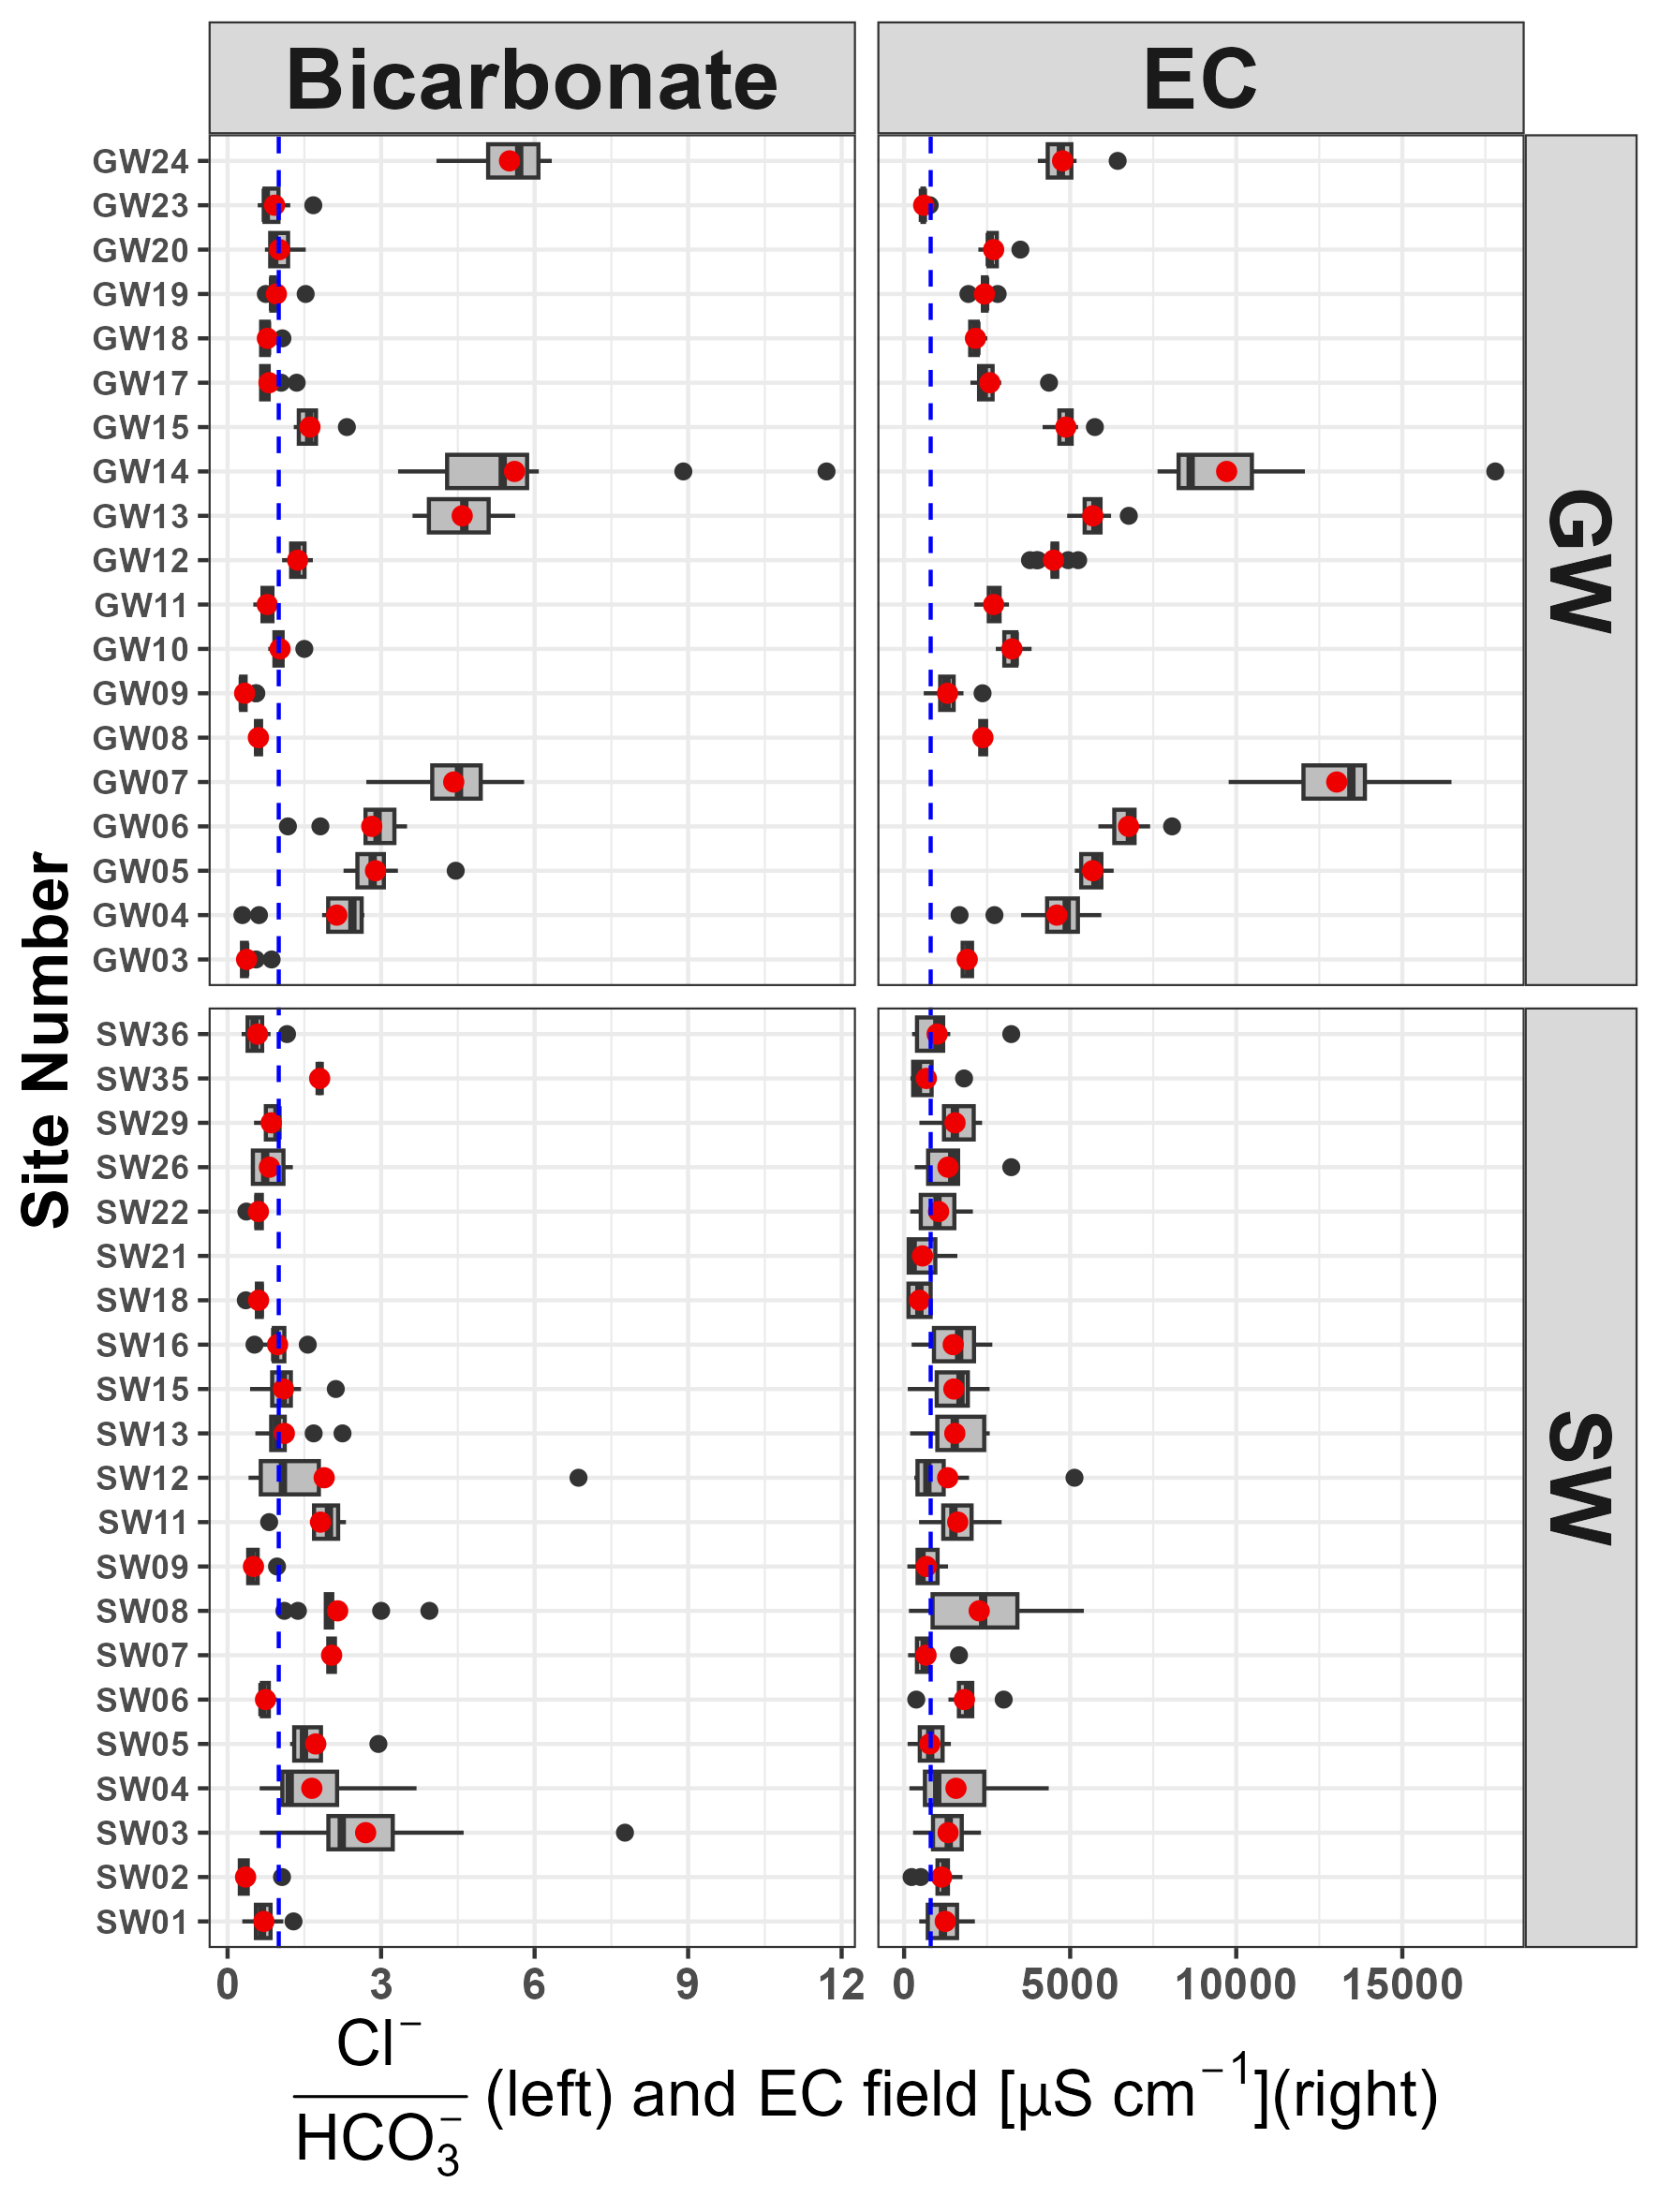
\includegraphics[width=0.7\linewidth]{Figures/boxplots} \caption{Variation across time of the $\mathrm{Cl:HCO_3}$ ratio (left) and EC (right) by sampling location represented as a boxplot. Only locations with more than 10 observations over the 14 years are included. The blue dashed line (left) indicates a $\mathrm{Cl:HCO_3}$ ratio of 1, while the blue dashed line (right) is the drinking water limit of 800 $\mathrm{\mu S~cm^{-1}}$.}\label{fig:boxplots}
\end{figure}

There is clear spatial variation in water parameters throughout the
catchment, including between groundwater and surface water sampling
sites (Figure \ref{fig:spatial-map}). As examples, the spatial
distributions for EC and Cl:HCO\textsubscript{3} are shown for sample
sites with more than 10 observations over the sampling period. Similar
maps can be easily generated for other parameters using the code in the
markdown document. In the map, the concentration is indicated by the
size of the symbol, while the colour shading indicates the variability.
This suggests surface water samples had lower variability and lower salt
concentrations. In addition, samples on the North western side of the
catchment had higher salt concentrations and higher
Cl:HCO\textsubscript{3} ratios, which is also associated with higher
variance in the samples.

Below the maps, boxplots (Figure \ref{fig:boxplots}) highlight the
difference in the distributions between the surface water sample sites
and the groundwater sample sites. For sites that have more than 10
observations, this highlights the difference between sample sites,
reflected spatially on the maps. For example, it highlights that high EC
sites also tended to have high Cl:HCO\textsubscript{3} values, and
conversely that low salinity groundwater tended to be associated with
low Cl:HCO\textsubscript{3} values. It also points out the single well
(GW23) that has a very low EC. Previous studies have suggested there may
be a difference in Cl:HCO\textsubscript{3} ratio in surface water
between the eastern and western parts of the Muttama catchment
\citep{Conyers2008}, and Figure \ref{fig:spatial-map} suggest a similar
pattern, with samples in the North and West being higher in EC and high
in Cl:HCO\textsubscript{3} values, while the Eastern and Southern areas
have lower variability in the surface water samples and lower
Cl:HCO\textsubscript{3} values.

\begin{figure}
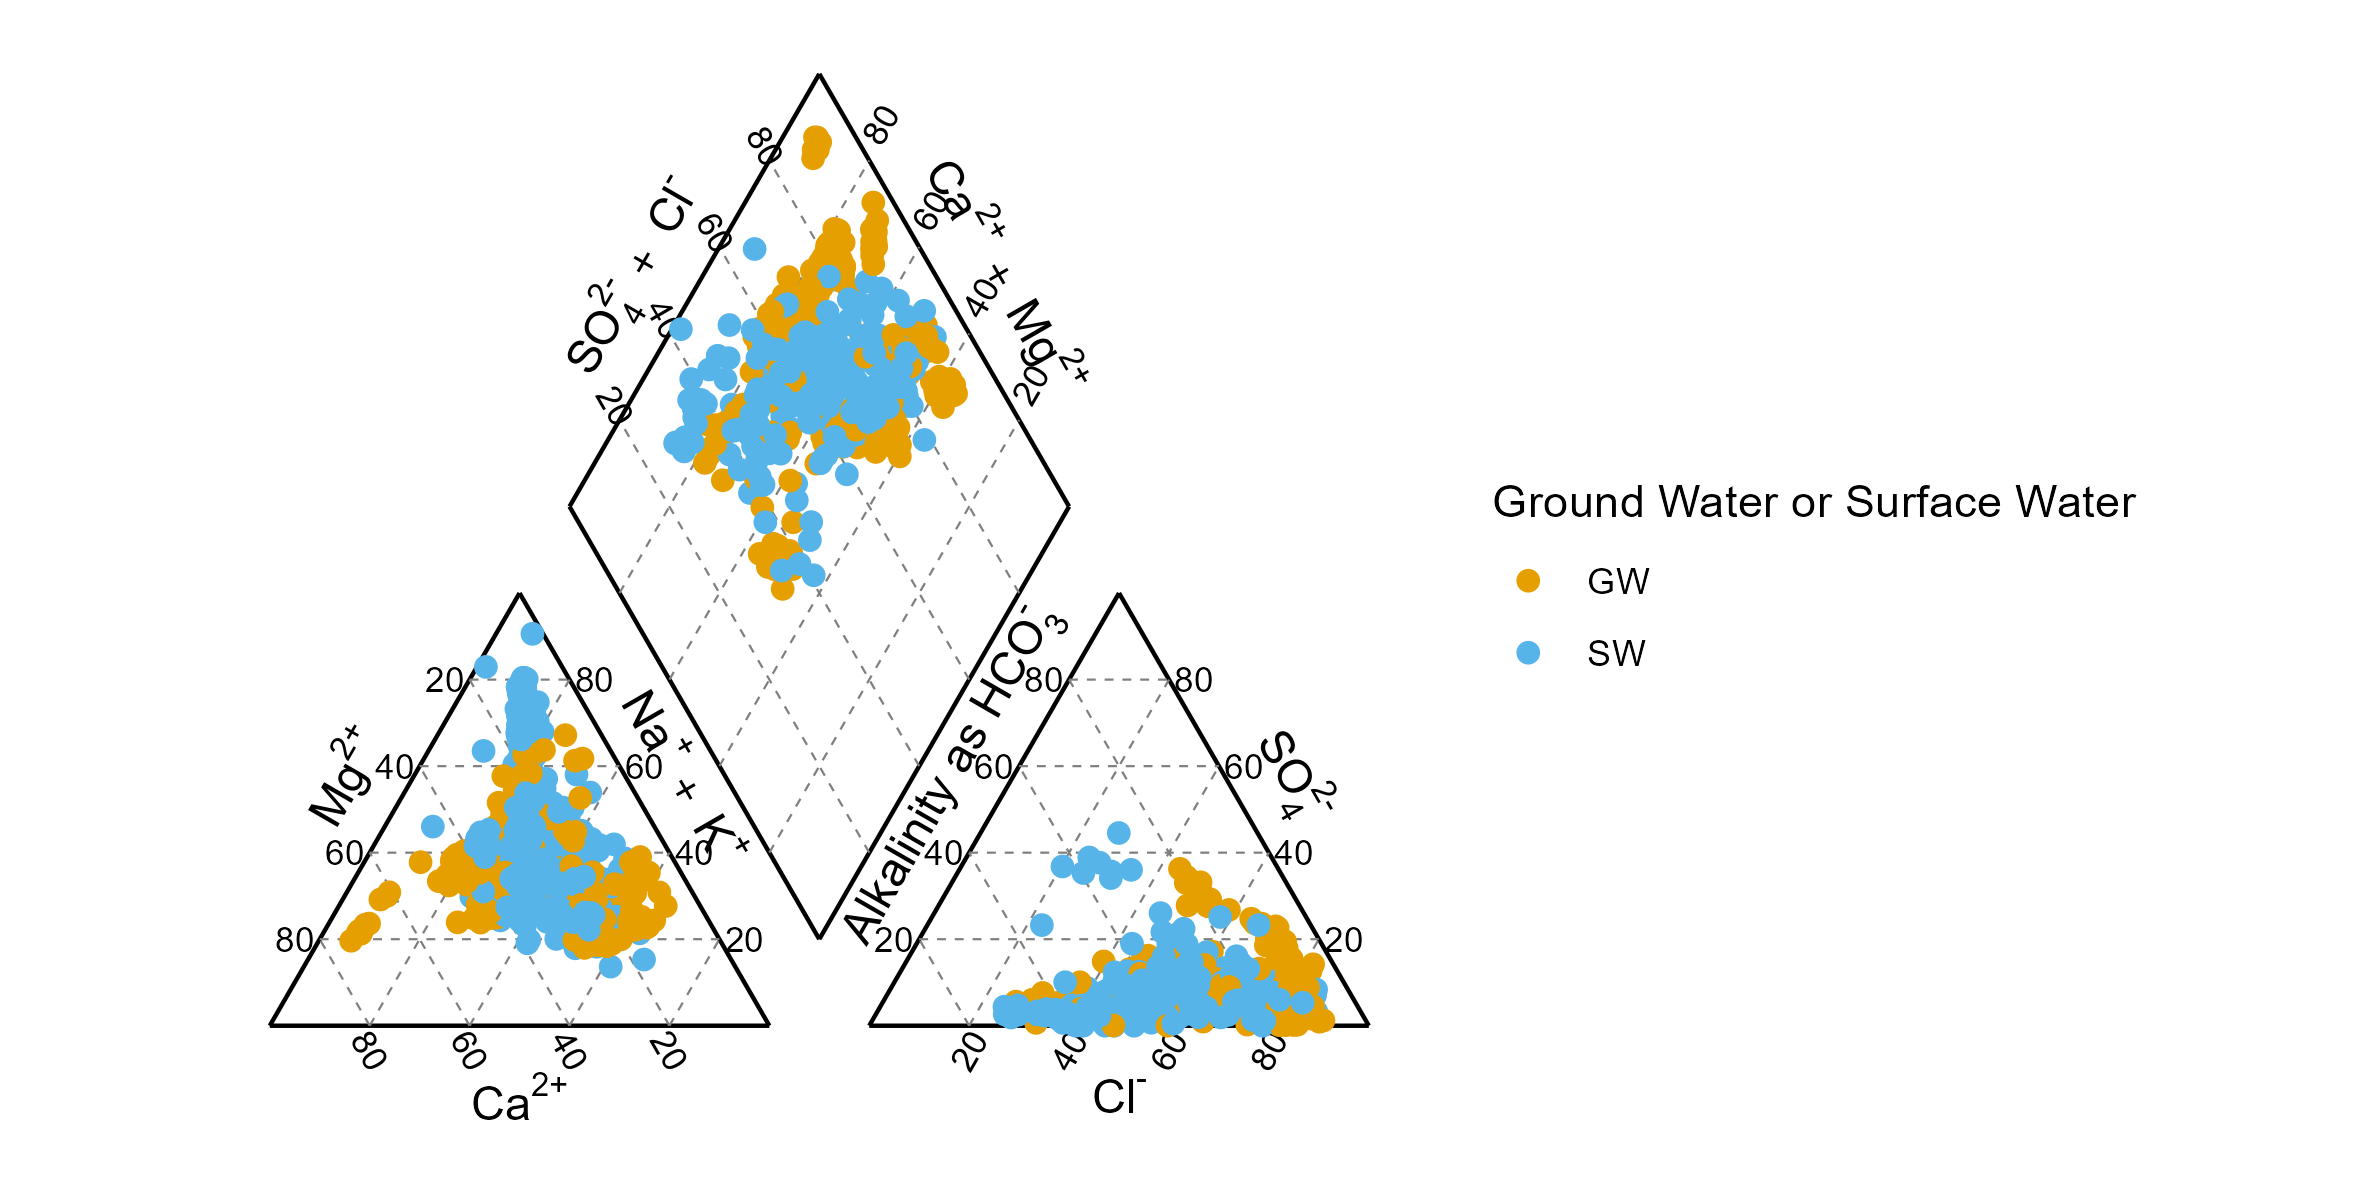
\includegraphics[width=1\linewidth]{Figures/piper_plot} \caption{Piper-plot of all groundwater and surface water data collected over the period with complete major anion data.}\label{fig:piperplot}
\end{figure}

\subsection{Piper plot}

The piper plot contains the data for all the samples with complete major
anion and cation data, which are 500 samples. Of these, 229 are surface
water samples and the rest groundwater samples. The piper plot of the
data (Figure \ref{fig:piperplot}) does not provide much clarity as the
samples cover a large area across the ternary space. There is a slight
shift towards the HCO\textsubscript{3} and Ca/Mg type waters for the
groundwater samples compared to the surface water samples, which are
more Na dominated. There is also a small cluster of surface water
samples that are more SO\textsubscript{4} dominated, potentially
indicating different geological origins as mentioned earlier in the
paper. However, some of the groundwater samples are very high in Cl,
explaining the high EC values observed for these samples.

\section{Discussion}

The dataset in this paper is unique in Australia. There are surface
water and groundwater geochemistry datasets from experimental small
catchments \citep[i.e.][]{Hughes2007, crosbie2007, Summerell2006}, but
not many of these are publicly or easily accessible. In contrast, there
are data from very large state and national datasets
\citep[i.e.][]{Jolly2001, thorslund_vanvliet2020}, but there are limited
publicly available data sets that cover similar substantial space and
time scales, and the range of hydrogeochemistry covered here. This is
particularly true in the case of shallow groundwater (\textless{} 20m)
which is the focus in this dataset.

As a baseline comparison, we compared the EC data from the catchment
samples with data from the global database from Thorslund and van Vliet
\citeyearpar{thorslund_vanvliet2020}. We subset the global database by
Australia, and restricted the groundwater data to shallow groundwater
\textless{} 20m from the surface (Figure \ref{fig:global-plot}). The
data from this figure are not included in the github due to the size of
the global data set and because the original data is readily available.
The figure clearly shows that the data collected in the Muttama
catchment fall well within the overall distribution of comparable
observed salinity values in Australia for both surface water and
groundwater.

In addition, comparison with Table 3 and Figure 5 in \citet{Hughes2007}
clearly highlights the value of the Cl/HCO\textsubscript{3} ratio in
comparing values of EC, Cl, and HCO\textsubscript{3}. For example, in a
catchment about 100 km north of Muttama catchment, \citet{Hughes2007}
found a much lower mean of 77 mg L\textsuperscript{-1} for
CaCO\textsubscript{3} in runoff. This study found a higher mean of 334
mg L\textsuperscript{-1} (Table \ref{tab:TableElementstats}). However,
\citet{Hughes2007} found a mean of 1056 mg L\textsuperscript{-1} for Cl,
while this study found a much lower mean of 294 mg
L\textsuperscript{-1}, suggesting quite different ratios. Finally,
\citet{Hughes2007} reported a mean EC of 3717 \(\mu S/cm\) in runoff,
while our data has mean of 1246 \(\mu S/cm\) (using the temperature
corrected value). In other words, the EC values in the Muttama Creek
catchment are more dominated by the alkalinity, resulting in lower EC
values. However, similar to Muttama Creek catchment, \citet{Hughes2007}
also indicates much higher alkalinity in the groundwater.

\begin{figure}
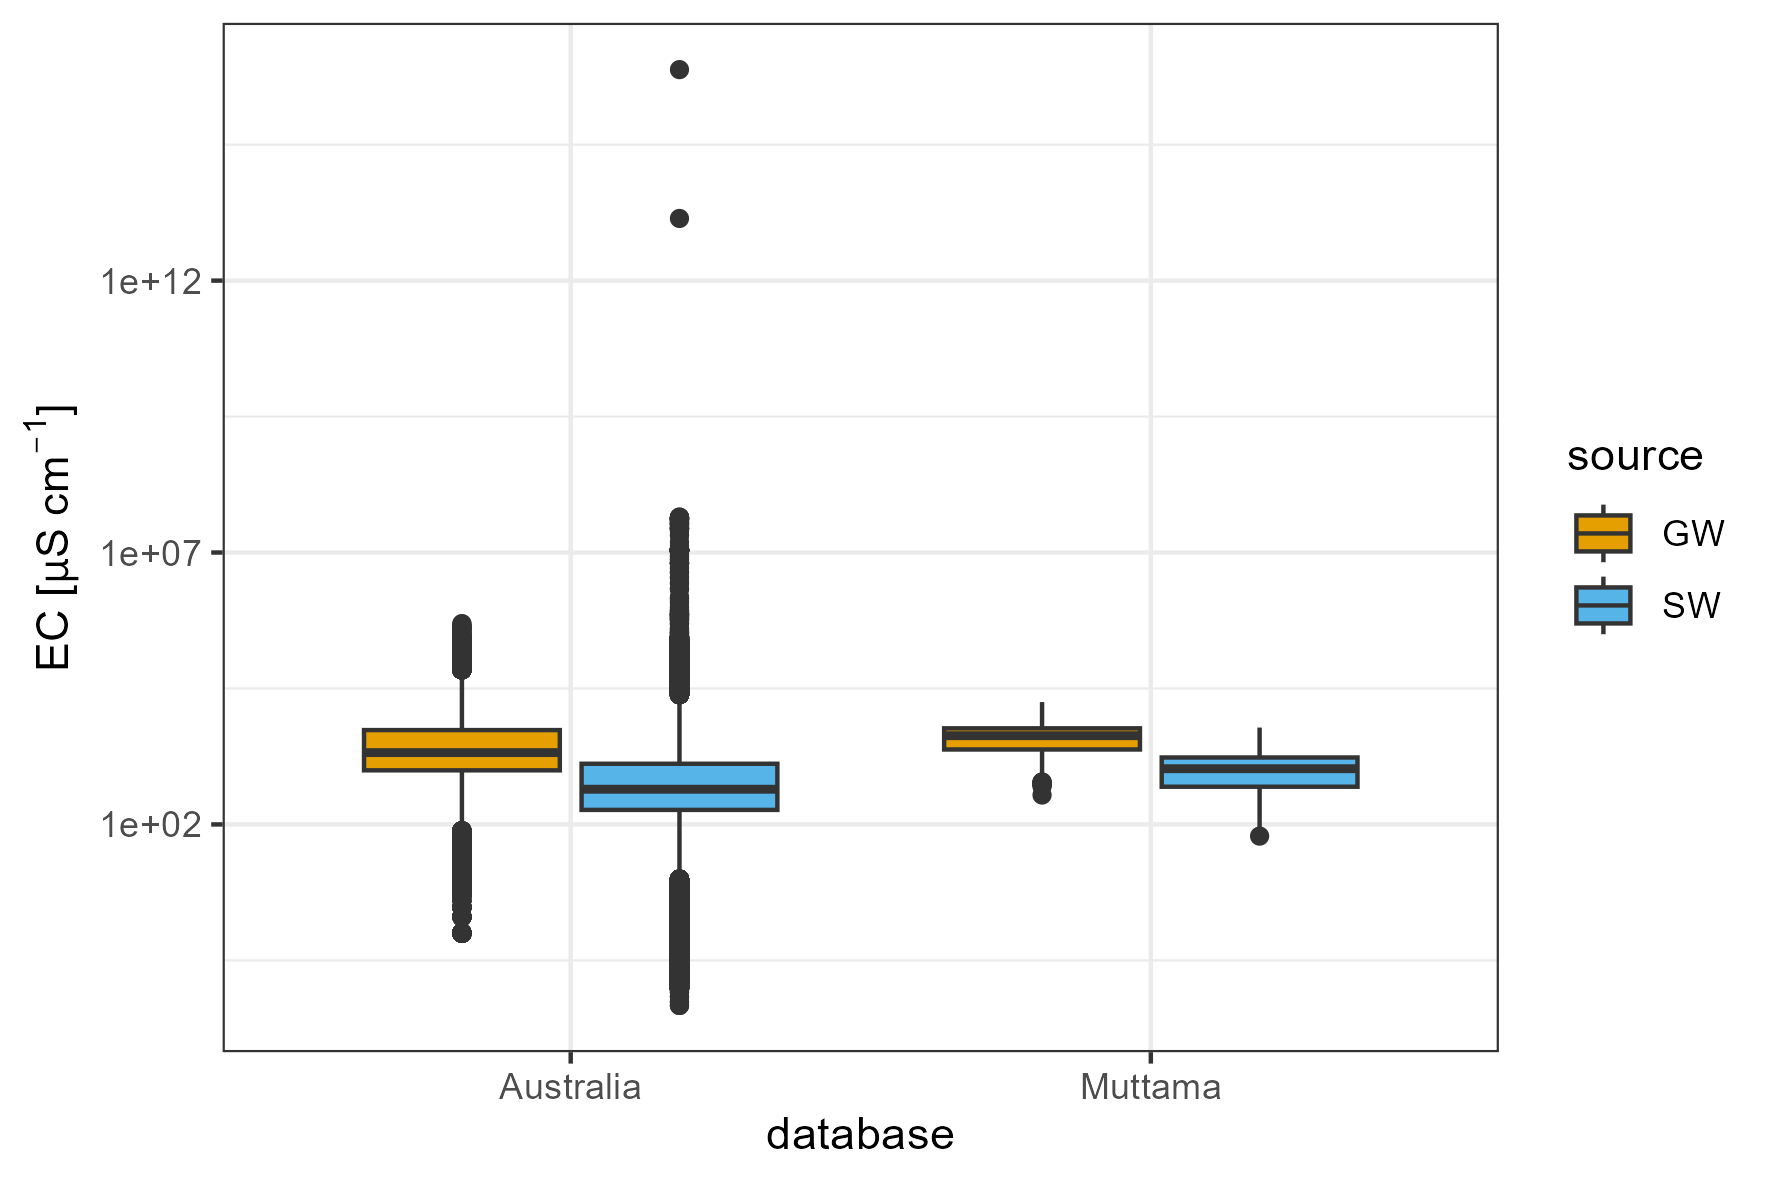
\includegraphics[width=0.8\linewidth]{Figures/globalboxplot} \caption{Boxplots comparing the electrical conductivity for samples of the Australian database extracted from Thorslund and van Vliet (2020) and the database of samples from Muttama Catchment.}\label{fig:global-plot}
\end{figure}

The Muttama catchment dataset presented here covers multiple sites,
multiple time periods and multiple sampling campaigns. Despite the
strengths of this dataset (i.e., the large spatial and temporal range
and large range in hydrogeochemical parameters), there are also
limitations. As the groundwater data clearly shows, the actual number of
possible sample sites is limited by the existing and accessible
groundwater wells. Over the 14 years of research, several groundwater
wells were accidentally destroyed during farm operations, further
reducing the sample opportunities. The number of surface water sampling
sites in the catchment is limited by the ephemeral nature of the stream
network, with some creeks not flowing for long periods. The overall
sampling is therefore limited in scope, as is clearly shown in the
spatial maps (Figure \ref{fig:spatial-map}).

The development of the dataset over many years regrettably does not
allow a full uncertainty analysis. There is reasonable quality
assessment of the laboratory analysis of the samples taken by
\citet{Akter2018} (see the appendices in \citet{Akter2018}), there is
less reporting of this for the other samples. An exception to this is
the samples analysed by the commercial laboratory, where a strict
quality protocol was followed. Some uncertainty can be gleaned from the
mass balance closure of the major cations for the laboratory analysis.
None of this provides an understanding of the uncertainty associated
with the field measurements and the potential manual handling errors.
Despite these potential sources of uncertainty, the analysis in this
paper highlights the spatial and temporal consistency of the data, thus
providing evidence of manageable uncertainty in overall dataset.
Therefore, the dataset is valuable in the general space time information
that it provides.

The dataset suggests implications for management of salinity in the
Muttama catchment. The samples clearly indicate that the main source of
high Cl salinity originates from the sediments and rocks on the
northwestern side of the catchment. This is further complicated by the
artesian nature of some of the wells in this area. However, as the water
level data and \citet{Akter2021} has highlighted, the shallow
groundwater levels and concentrations only partly respond to rainfall
recharge. Investment and incentives to reduce recharge should focus on
these areas, particularly to limit the movement of saline discharge into
the creek \citep{Akter2018}.

The presented dataset provides significant opportunities for further
research, particularly because of the length of the time series. For
example, there is the opportunity to examine trends in salinity due to
changes in climate. There are few datasets that cover shallow
groundwater and concurrent surface water across a similar wide range of
hydrogeochemistry. This opens up the opportunity to look at temporal
variability in groundwater surface water connections, particularly for
flat semi-arid systems similar to Muttama Catchment, as was done for a
more limited set of data in \citet{Akter2018}.

The comprehensive nature of the data also creates opportunities for
testing more complex hydrological and hydrogeological models. An example
could be to extend the work by Deb et al.
\citeyearpar{debMuttamamodel2019} to look at variations in
rainfall-runoff response during wet and dry periods, which for Muttama
catchment was linked to groundwater surface water connections. Finally,
given our intention to continue collecting data in the catchment, there
is an opportunity to look at shifts in the hydrogeochemistry as a result
of wet and dry periods.

\section{Conclusions}

Detailed datasets for medium to large scale catchments (greater or equal
than 1000 km\textsuperscript{2}) are underrepresented in salinity
research in Australia and worldwide, with very few public datasets
identified for Australia. This paper reports on a long term (14 year)
hydrogeochemistry dataset from a single medium scale catchment
(\textgreater{} 1000 km\textsuperscript{2}) in NSW, Australia. This
dataset includes a total of 1160 water samples from 62 locations within
the catchment and includes groundwater and surface water sites. While
the dataset was collected by different groups of people at different
times and locations, it still provides a valuable long term and
spatially diverse data set. The complete sample set covers a wide range
of flow and wetness conditions. Clear differences were observed in pH,
electroconductivity, and in ion ratios between groundwater and surface
water samples. Spatial differences in water chemistry are also apparent,
with our data reinforcing prior chemical gradients observed in the
catchment. Though in this paper we only provide a limited analysis of
the data, we anticipate the dataset can be used for research to gain
better insight into the spatio-temporal evolution of hydrogeochemical
processes from larger catchments and improve the understanding of
catchment salinity.

\bigskip

\competinginterests{The authors declare no competing interests}.

\bigskip

\noindent \textbf{Availability code \& data}

\begin{itemize}
\tightlist
\item
  The majority of the code and associated data, including the Rmarkdown
  for this paper, is stored on Github
  \url{https://github.com/WillemVervoort/MuttamaDataPaper}.\\
\item
  The hydrogeochemistry data is located on
  \href{doi.org/10.25910/m0wp-8890}{the University of Sydney
  escholarship repository} \citet{vervoort2025}.\\
\item
  However, due to the volume of raw data, the groundwater logger data is
  stored in a separate Open Science Foundation project:
  \url{https://doi.org/10.17605/OSF.IO/BEUWK} \citet{vervoort2024}.
\end{itemize}

\bigskip

\noindent \textbf{Author contributions}\\
TB initiated the sampling campaign. TB, FvO, FD and RWV conceptualised
the overall study, and managed the project. RWV and MT wrote the draft
paper and analysed results. FA, DK and JL collected and analysed the
majority of the samples. MT, AB, JM, FA and DK analysed and managed the
data. All authors participated in sampling, laboratory analysis and
review of the paper.

\bigskip

\noindent \textbf{Acknowledgements}\\
This dataset would not have been possible without the generous
assistance and access to properties from the following land owners in
the Muttama Creek area: R. Last, the Tozer family, M. Sullivan, P.
McClintock, P. McGuire, S. Sharman, A. Hollihan, the managers at Brawlin
Springs as part of the Romani Pastoral Company, and the managers and
owners of Wavehill, in particular J. Litchfield. We would like to thank
several generations of students in the units LWSC2002, ENVX3003 and
ENSY5708, as well a multiple interns from French Institutions and
Wageningen University for assisting with the sample collection.






%%%%%%%%%%%%%%%%%%%%%%%%%%%%%%%%%%%%%%%%%%
%% optional

%%%%%%%%%%%%%%%%%%%%%%%%%%%%%%%%%%%%%%%%%%

%%%%%%%%%%%%%%%%%%%%%%%%%%%%%%%%%%%%%%%%%%

%%%%%%%%%%%%%%%%%%%%%%%%%%%%%%%%%%%%%%%%%%
\competinginterests{} %% this section is mandatory even if you declare that no competing interests are present

%%%%%%%%%%%%%%%%%%%%%%%%%%%%%%%%%%%%%%%%%%

%%%%%%%%%%%%%%%%%%%%%%%%%%%%%%%%%%%%%%%%%%

%% REFERENCES
%% DN: pre-configured to BibTeX for rticles

%% The reference list is compiled as follows:
%%
%% \begin{thebibliography}{}
%%
%% \bibitem[AUTHOR(YEAR)]{LABEL1}
%% REFERENCE 1
%%
%% \bibitem[AUTHOR(YEAR)]{LABEL2}
%% REFERENCE 2
%%
%% \end{thebibliography}

%% Since the Copernicus LaTeX package includes the BibTeX style file copernicus.bst,
%% authors experienced with BibTeX only have to include the following two lines:
%%
\bibliographystyle{copernicus}
\bibliography{datapaper.bib}
%%
%% URLs and DOIs can be entered in your BibTeX file as:
%%
%% URL = {http://www.xyz.org/~jones/idx_g.htm}
%% DOI = {10.5194/xyz}


%% LITERATURE CITATIONS
%%
%% command                        & example result
%% \citet{jones90}|               & Jones et al. (1990)
%% \citep{jones90}|               & (Jones et al., 1990)
%% \citep{jones90,jones93}|       & (Jones et al., 1990, 1993)
%% \citep[p.~32]{jones90}|        & (Jones et al., 1990, p.~32)
%% \citep[e.g.,][]{jones90}|      & (e.g., Jones et al., 1990)
%% \citep[e.g.,][p.~32]{jones90}| & (e.g., Jones et al., 1990, p.~32)
%% \citeauthor{jones90}|          & Jones et al.
%% \citeyear{jones90}|            & 1990


\end{document}
